% !TEX program = xelatex
\documentclass[12pt, a4paper]{article}

% ============================================================
%  Page Layout
% ============================================================
\usepackage[
    paperwidth=210mm, paperheight=297mm,
    left=22mm, right=22mm, top=28mm, bottom=28mm,
    headheight=14.5pt, headsep=6mm, footskip=10mm,
    columnsep=20pt
]{geometry}

% ============================================================
%  Chinese Support (XeLaTeX + Ubuntu fonts)
% ============================================================
\usepackage[fontset=ubuntu]{ctex}

% ============================================================
%  Mathematics
% ============================================================
\usepackage{amsmath, amssymb, mathtools}
\usepackage{bm}

% ============================================================
%  Tables
% ============================================================
\usepackage{booktabs}
\usepackage{multirow}
\usepackage{array}
\usepackage{adjustbox}
\newcolumntype{C}[1]{>{\centering\arraybackslash}p{#1}}

% ============================================================
%  Figures & Graphics
% ============================================================
\usepackage{graphicx}
\usepackage{float}
\usepackage{caption}
\usepackage{subcaption}
\captionsetup[figure]{
    font={small}, labelfont={bf},
    labelsep=period, justification=centering, skip=8pt
}
\captionsetup[table]{
    font={small}, labelfont={bf},
    labelsep=period, justification=centering, skip=6pt
}

% ============================================================
%  TikZ & PGFPlots
% ============================================================
\usepackage{tikz}
\usetikzlibrary{
    shapes.geometric, arrows.meta, positioning,
    calc, patterns, fit, decorations.pathreplacing,
    backgrounds
}
\usepackage{pgfplots}
\pgfplotsset{compat=1.18}
\usepgfplotslibrary{groupplots}

% Journal-standard color palette
\definecolor{cBlue}{HTML}{2171B5}
\definecolor{cRed}{HTML}{CB181D}
\definecolor{cGreen}{HTML}{238B45}
\definecolor{cOrange}{HTML}{F16913}
\definecolor{cPurple}{HTML}{6A51A3}
\definecolor{cGray}{HTML}{636363}
\definecolor{cLightGray}{HTML}{D9D9D9}

% ============================================================
%  Typography
% ============================================================
\usepackage{setspace}
\setstretch{1.35}
\usepackage{indentfirst}
\setlength{\parindent}{1.5em}
\setlength{\parskip}{0pt plus 1pt}
\usepackage{enumitem}
\setlist{nosep, leftmargin=1.8em}
\usepackage{microtype}

% ============================================================
%  Running Headers & Footers (after cover)
% ============================================================
\usepackage{fancyhdr}

% ============================================================
%  Algorithm
% ============================================================
\usepackage[ruled, linesnumbered, vlined]{algorithm2e}
\SetAlFnt{\small}
\SetAlCapFnt{\small}
\SetAlCapNameFnt{\small}
\SetKwInput{KwHyper}{Hyperparameters}

% ============================================================
%  Hyperlinks
% ============================================================
\usepackage{hyperref}
\hypersetup{
    colorlinks=true,
    linkcolor=cBlue!80!black,
    citecolor=cGreen!70!black,
    urlcolor=cBlue!70!black,
    bookmarksnumbered=true, pdfstartview=FitH
}

% ============================================================
%  Bibliography
% ============================================================
\usepackage[
    backend=biber, style=numeric-comp,
    sorting=none, maxnames=3, minnames=1,
    giveninits=true, doi=false, isbn=false, url=false
]{biblatex}

\begin{filecontents}{\jobname.bib}
@inproceedings{hatamizadeh2022swin,
  author    = {Hatamizadeh, Ali and Tang, Yucheng and Nath, Vishwesh and Yang, Dong and Myronenko, Andriy and Landman, Bennett and Roth, Holger R. and Xu, Daguang},
  title     = {{Swin UNETR}: Swin Transformers for Semantic Segmentation of Brain Tumors in {MRI} Images},
  booktitle = {Int.\ Conf.\ Medical Image Computing and Computer-Assisted Intervention (MICCAI)},
  pages     = {272--282}, year = {2022}, publisher = {Springer}
}
@inproceedings{ronneberger2015unet,
  author    = {Ronneberger, Olaf and Fischer, Philipp and Brox, Thomas},
  title     = {{U-Net}: Convolutional Networks for Biomedical Image Segmentation},
  booktitle = {Int.\ Conf.\ Medical Image Computing and Computer-Assisted Intervention (MICCAI)},
  pages     = {234--241}, year = {2015}, publisher = {Springer}
}
@inproceedings{liu2021swin,
  author    = {Liu, Ze and Lin, Yutong and Cao, Yue and Hu, Han and Wei, Yixuan and Zhang, Zheng and Lin, Stephen and Guo, Baining},
  title     = {Swin Transformer: Hierarchical Vision Transformer using Shifted Windows},
  booktitle = {IEEE/CVF Int.\ Conf.\ Computer Vision (ICCV)},
  pages     = {10012--10022}, year = {2021}
}
@inproceedings{lin2017focal,
  author    = {Lin, Tsung-Yi and Goyal, Priya and Girshick, Ross and He, Kaiming and Doll{\'a}r, Piotr},
  title     = {Focal Loss for Dense Object Detection},
  booktitle = {IEEE Int.\ Conf.\ Computer Vision (ICCV)},
  pages     = {2980--2988}, year = {2017}
}
@article{cardoso2022monai,
  author    = {Cardoso, M. J. and Li, W. and Brown, R. and Ma, N. and Kerfoot, E. and Wang, Y. and others},
  title     = {{MONAI}: An open-source framework for deep learning in healthcare},
  journal   = {arXiv preprint arXiv:2211.02701}, year = {2022}
}
@article{isensee2021nnunet,
  author    = {Isensee, F. and Jaeger, P. F. and Kohl, S. A. A. and Petersen, J. and Maier-Hein, K. H.},
  title     = {{nnU-Net}: a self-configuring method for deep learning-based biomedical image segmentation},
  journal   = {Nature Methods}, volume = {18}, number = {2}, pages = {203--211}, year = {2021}
}
@inproceedings{wang2022uctransnet,
  author    = {Wang, H. and Cao, P. and Wang, J. and Zaiane, O. R.},
  title     = {{UCTransNet}: Rethinking the Skip Connections in {U-Net} from a Channel-wise Perspective with Transformer},
  booktitle = {AAAI Conf.\ Artificial Intelligence}, year = {2022}
}
@article{chen2021transunet,
  author    = {Chen, J. and Lu, Y. and Yu, Q. and Luo, X. and Adeli, E. and Wang, Y. and Lu, L. and Yuille, A. L. and Zhou, Y.},
  title     = {{TransUNet}: Transformers Make Strong Encoders for Medical Image Segmentation},
  journal   = {arXiv preprint arXiv:2102.04306}, year = {2021}
}
@article{loshchilov2017decoupled,
  author    = {Loshchilov, I. and Hutter, F.},
  title     = {Decoupled Weight Decay Regularization},
  journal   = {arXiv preprint arXiv:1711.05101}, year = {2017}
}
@inproceedings{milletari2016v,
  author    = {Milletari, F. and Navab, N. and Ahmadi, S.-A.},
  title     = {{V-Net}: Fully Convolutional Neural Networks for Volumetric Medical Image Segmentation},
  booktitle = {Int.\ Conf.\ 3D Vision (3DV)}, pages = {565--571}, year = {2016}
}
@inproceedings{zhou2018unetpp,
  author    = {Zhou, Zongwei and Rahman Siddiquee, Md Mahfuzur and Tajbakhsh, Nima and Liang, Jianming},
  title     = {{UNet++}: A Nested {U-Net} Architecture for Medical Image Segmentation},
  booktitle = {Deep Learning in Medical Image Analysis and Multimodal Learning for Clinical Decision Support (DLMIA)},
  pages     = {3--11}, year = {2018}, publisher = {Springer}
}
@inproceedings{tan2019efficientnet,
  author    = {Tan, Mingxing and Le, Quoc V.},
  title     = {{EfficientNet}: Rethinking Model Scaling for Convolutional Neural Networks},
  booktitle = {Int.\ Conf.\ Machine Learning (ICML)}, year = {2019}
}
\end{filecontents}
\addbibresource{\jobname.bib}

% ============================================================
%  Custom Commands
% ============================================================
\newcommand{\mrm}[1]{\mathrm{#1}}
\newcommand{\Dice}{\mrm{Dice}}
\newcommand{\IoU}{\mrm{IoU}}
\newcommand{\mDSC}{\mrm{mDSC}}
\newcommand{\mIoU}{\mrm{mIoU}}
\newcommand{\Focal}{\mrm{Focal}}
\newcommand{\R}{\mathbb{R}}

% ============================================================
\begin{document}
% ============================================================

% ============================================================
% 封面 Cover Page
% ============================================================
\thispagestyle{empty}
\begin{center}
    \vspace*{2cm}
    {\Huge \bfseries 《医学图像处理技术》期末项目报告} \\[2.5cm]

    \begin{flushleft}
        \hspace*{2cm}
        \begin{minipage}{0.9\textwidth}
            {\large \bfseries 题目：\underline{任务二 Chest CT Segmentation}} \\[1cm]

            {\large \bfseries 组号：\underline{15}} \\[0.6cm]

            {\large \bfseries 小组成员姓名：\underline{俞烨，张天硕，张璟文，张鸿榜，} \\
            \underline{吴君凯，黄绍华，陈飞翔，刘华胜}} \\[0.6cm]

            {\large \bfseries 小组成员学号：\underline{102301116，102301113，102301114，102301115，} \\
            \underline{102301121，102301137，102301142，022304111}} \\[0.8cm]

            {\large \bfseries 评分：} \\[0.4cm]

            {\normalsize 1、\bfseries 语言与排版（25分）：} \rule{8cm}{0.4pt} \\[0.4cm]

            {\normalsize 2、\bfseries 问题难易程度（25分）：} \rule{8cm}{0.4pt} \\[0.4cm]

            {\normalsize 3、\bfseries 实践掌握程度（50分）：} \rule{8cm}{0.4pt} \\[0.4cm]

            {\large \bfseries 总分：} \rule{12cm}{0.4pt}
        \end{minipage}
    \end{flushleft}
\end{center}
\clearpage

% ============================================================
% English Abstract
% ============================================================
\thispagestyle{empty}

\begin{center}
\begin{minipage}{0.9\textwidth}
\textbf{Abstract:}Multi-organ segmentation of chest CT images constitutes a critical component of computer-aided diagnosis systems, with significant clinical implications for lung disease screening, cardiac function assessment, and airway pathology analysis. This study systematically compares multiple architectures for chest CT multi-organ segmentation on the Kaggle Chest CT Segmentation dataset. A reference baseline is first established using the dataset provider's open-source U-Net implementation with an EfficientNet-B2 encoder and BCEDiceLoss, achieving a validation Dice coefficient of 0.968. Subsequently, two architectures are investigated: Swin-UNETR~v2, which employs a hierarchical Swin Transformer encoder to extract multi-scale global features with a U-Net-style decoder, and UNet++ with a pretrained EfficientNet-B2 encoder and nested skip pathways.

During training, the DiceFocalLoss composite loss function is adopted to alleviate class imbalance, combined with the AdamW optimizer and cosine annealing learning rate scheduling. Three independent training runs were conducted: a baseline experiment and a parameter optimization experiment using Swin-UNETR~v2 (200 epochs each), and a comparative experiment using UNet++ (150 epochs). The best Swin-UNETR~v2 model from the parameter optimization experiment achieves a mean Dice coefficient of 0.9390 on the test set, with per-organ Dice scores of up to 0.9664 for lung, 0.9054 for heart, and 0.9458 for trachea. The UNet++ model achieves the highest mean Dice coefficient of 0.9661, with per-organ Dice scores of 0.9702 for lung, 0.9718 for heart, and 0.9563 for trachea.

Experimental results demonstrate that the pretrained CNN encoder architecture effectively captures semantic features of organs at varying scales in chest CT images, achieving performance comparable to the reference baseline and superior to the Transformer-based approach trained from scratch. This report provides comprehensive details on the methodology, implementation, training dynamics, and results analysis, along with complete experimental records and visualization examples.

\vspace{1cm}
\centering \textbf{Keywords:} Chest CT, Multi-organ Segmentation, Swin-UNETR, DiceFocalLoss, Medical Image Analysis
\end{minipage}
\end{center}

\clearpage

% ============================================================
% Chinese Abstract
% ============================================================
\thispagestyle{empty}

\begin{center}
\begin{minipage}{0.9\textwidth}
\textbf{摘要：}胸部CT图像多器官分割是计算机辅助诊断系统的核心环节，对肺部疾病筛查、心脏功能评估及气道病变分析具有重要临床意义。本研究在Kaggle Chest CT Segmentation数据集上系统比较了多种架构的胸部CT多器官分割性能。首先以数据集提供方的开源U-Net实现（EfficientNet-B2编码器 + BCEDiceLoss）建立参考基线，其验证集Dice系数达0.968。随后研究了两种架构：Swin-UNETR~v2以Swin Transformer层级编码器提取多尺度全局特征，经U-Net式解码器与跳跃连接逐步恢复空间分辨率；UNet++采用预训练EfficientNet-B2编码器与嵌套跳跃路径解码器。

训练阶段采用DiceFocalLoss复合损失函数缓解类别不平衡问题，配合AdamW优化器与余弦退火学习率调度策略，进行了三组独立实验：基于Swin-UNETR~v2的基准实验与参数优化实验（各200轮），以及基于UNet++的对比实验（150轮）。参数优化实验的最优Swin-UNETR~v2模型在测试集上取得了0.9390的平均Dice系数（mDSC），肺部分割Dice系数最高达0.9664，心脏0.9054，气管0.9458。UNet++模型取得了最高的0.9661平均Dice系数，肺、心脏、气管的DSC分别为0.9702、0.9718和0.9563。

实验结果表明，预训练CNN编码器架构能够有效捕获胸部CT图像中不同尺度器官的语义特征，其性能与参考基线相当且显著优于从头训练的Transformer架构。本报告详细阐述了研究方法、实现过程、训练动态和结果分析，提供了完整的实验记录和可视化示例。

\vspace{1cm}
\centering \textbf{关键词：} 胸部CT；多器官分割；Swin-UNETR；DiceFocalLoss；医学图像分析
\end{minipage}
\end{center}

\clearpage

% ============================================================
% Enable Headers for Main Content
% ============================================================
\pagestyle{fancy}
\fancyhf{}
\fancyhead[L]{\small\textit{任务二 Chest CT Segmentation}}
\fancyhead[R]{\small\textit{期末项目报告}}
\fancyfoot[C]{\thepage}
\renewcommand{\headrulewidth}{0.3pt}
\renewcommand{\footrulewidth}{0pt}

\setcounter{page}{1}

% ============================================================
% Table of Contents
% ============================================================
\tableofcontents
\clearpage

% ============================================================
\section{引言}
\label{sec:intro}
% ============================================================

胸部计算机断层扫描（Computed Tomography, CT）是临床胸部疾病诊断最常用的影像学检查手段，其高分辨率横断面成像能够清晰显示肺部、心脏及气道等关键解剖结构~\cite{hatamizadeh2022swin}。精确的器官分割是后续定量分析与计算机辅助诊断（Computer-Aided Diagnosis, CAD）系统的基础，在以下场景中具有重要应用价值：（1）肺部疾病诊断，如肺结节检测、肺气肿量化与肺炎范围评估；（2）心脏功能评估，包括心室体积测量与心壁厚度分析；（3）气道病变分析，如气管狭窄与支气管扩张评估；（4）胸部手术规划与导航。

近年来，深度学习技术在医学影像分割领域取得了突破性进展。Ronneberger等人~\cite{ronneberger2015unet}提出的U-Net架构凭借编码器--解码器结构与跳跃连接，成为医学图像分割的里程碑方法。Isensee等人~\cite{isensee2021nnunet}提出的nnU-Net通过自适应配置策略进一步提升了分割性能。然而，基于卷积神经网络（CNN）的方法受限于局部感受野，难以建模长距离空间依赖关系。

为解决这一局限，Transformer架构逐渐被引入医学影像分割领域：Chen等人~\cite{chen2021transunet}提出TransUNet，将Transformer编码器与U-Net解码器级联；Wang等人~\cite{wang2022uctransnet}提出UCTransNet，在跳跃连接中引入通道注意力机制。Liu等人~\cite{liu2021swin}提出的Swin Transformer通过局部窗口自注意力与移位窗口机制，在保持线性计算复杂度的同时实现了高效的全局建模能力。Hatamizadeh等人~\cite{hatamizadeh2022swin}进一步提出Swin-UNETR，将Swin Transformer编码器与U-Net解码器深度融合，在多项医学分割基准上取得了领先性能。

尽管上述方法取得了显著进展，胸部CT多器官分割仍面临以下挑战：（1）器官形态变异大，个体间解剖差异显著；（2）小器官（如气管）像素占比低，类别不平衡问题突出；（3）器官边界模糊，相邻结构灰度差异小；（4）不同扫描设备与参数导致的图像质量差异影响模型泛化能力。

针对上述问题，本研究以数据集提供方的开源U-Net实现为参考基线，系统比较了Swin-UNETR~v2与UNet++两种架构在胸部CT多器官分割任务上的性能。Swin-UNETR~v2结合DiceFocalLoss复合损失函数与余弦退火学习率调度策略，在Kaggle Chest CT Segmentation数据集上实现了肺、心脏和气管三类器官的高精度分割；UNet++采用EfficientNet-B2预训练编码器与嵌套跳跃路径解码器，以更轻量的数据增强策略和更大的批大小进行训练，取得了更优的分割性能。

\subsection{主要贡献}
本研究的主要贡献包括：
\begin{enumerate}[leftmargin=2em, itemsep=4pt]
    \item 以数据集提供方的开源U-Net实现建立参考基线（val\_dice$\approx$0.968），为后续实验提供性能参照
    \item 采用Swin-UNETR~v2架构，充分利用Swin Transformer的全局建模能力与U-Net解码器的精确定位能力
    \item 引入UNet++（EfficientNet-B2编码器）作为对比模型，系统比较Transformer架构与CNN预训练编码器架构在胸部CT分割任务上的性能差异
    \item 引入DiceFocalLoss复合损失函数，有效缓解类别不平衡问题，提升小器官（气管）的分割性能
    \item 设计差异化的数据增强策略与训练配置，分析批大小、数据增强强度对模型收敛与泛化的影响
    \item 通过三次独立实验验证方法的有效性与参数优化的效果，最优模型（UNet++）取得0.9661的平均Dice系数，Swin-UNETR~v2最优达0.9390
    \item 提供完整的实现代码、训练记录和实验报告，便于后续研究复现与扩展
\end{enumerate}

\subsection{报告结构}
本报告其余部分安排如下：第2节介绍研究方法，包括参考基线、Swin-UNETR~v2与UNet++两种网络架构、数据预处理、损失函数与训练配置；第3节描述实验设置，包括数据集、环境配置、评价指标与实验设计；第4节展示实验结果并进行详细分析；第5节讨论两种架构的对比分析、与参考基线的对比、方法局限性与未来工作；最后第6节总结全文。

% ============================================================
\section{研究方法}
\label{sec:method}
% ============================================================

\subsection{参考基线}
\label{sec:baseline}

为建立性能参考基准，本研究首先复现了数据集提供方开源的U-Net实现（\texttt{exmaple.py}）作为参考基线。该实现采用\texttt{segmentation\_models\_pytorch}库的U-Net架构，以EfficientNet-B2~\cite{tan2019efficientnet}作为编码器，并加载ImageNet预训练权重。与本研究后续实验中使用的UNet++不同，该基线采用标准U-Net解码器，通过简单的跳跃连接将编码器特征与解码器特征拼接。

\subsubsection{训练配置}

参考基线的训练配置与本研究后续实验存在显著差异，具体如下：

\begin{table}[H]
    \centering
    \caption{参考基线训练配置}
    \label{tab:baseline_config}
    \begin{tabular}{@{}ll@{}}
        \toprule
        \textbf{超参数} & \textbf{值} \\
        \midrule
        架构 & U-Net (EfficientNet-B2编码器) \\
        编码器权重 & ImageNet预训练 \\
        损失函数 & BCEDiceLoss (BCE + Dice) \\
        优化器 & Adam (lr=$8{\times}10^{-5}$) \\
        学习率调度 & ReduceLROnPlateau (patience=3) \\
        批大小 & 8 \\
        训练轮数 & 100（预训练模型）+ 继续训练 \\
        随机种子 & 555 \\
        数据划分 & train\_test\_split (random\_state=69) \\
        数据增强 & VerticalFlip (p=0.5) + Normalize (ImageNet) \\
        框架 & albumentations + 自定义Dataset/Trainer \\
        \bottomrule
    \end{tabular}
\end{table}

\subsubsection{与本研究实验的关键差异}

参考基线与本研究后续实验在以下方面存在关键差异：（1）\textbf{架构}：基线采用标准U-Net，而非Swin-UNETR~v2或UNet++的嵌套跳跃路径设计；（2）\textbf{损失函数}：基线采用BCEDiceLoss（BCE与Dice的加权和），而非DiceFocalLoss，后者通过Focal机制对难分类样本赋予更高权重；（3）\textbf{优化器与调度器}：基线采用Adam优化器配合ReduceLROnPlateau调度器（验证指标停滞时降低学习率），而本研究采用AdamW配合CosineAnnealingLR（周期性余弦退火）；（4）\textbf{数据增强}：基线仅使用垂直翻转与归一化，增强策略远轻于Swin-UNETR~v2的完整增强管线；（5）\textbf{数据划分}：基线使用random\_state=69划分数据，与本研究后续实验的random\_state=520不同，导致训练/验证集样本构成存在差异；（6）\textbf{框架}：基线基于albumentations与自定义Dataset/Trainer类实现，而本研究基于MONAI框架构建。

这些差异使得参考基线与本研究实验之间的直接对比需考虑方法学差异，但基线仍为评估本研究方法的性能水平提供了重要参考。

\subsubsection{U-Net架构详解}

参考基线采用的U-Net架构~\cite{ronneberger2015unet}是医学图像分割领域的经典方法，其核心结构如图~\ref{fig:unet_arch}所示。U-Net采用对称的编解码结构，包含四个下采样阶段和四个上采样阶段：

\begin{figure}[H]
    \centering
    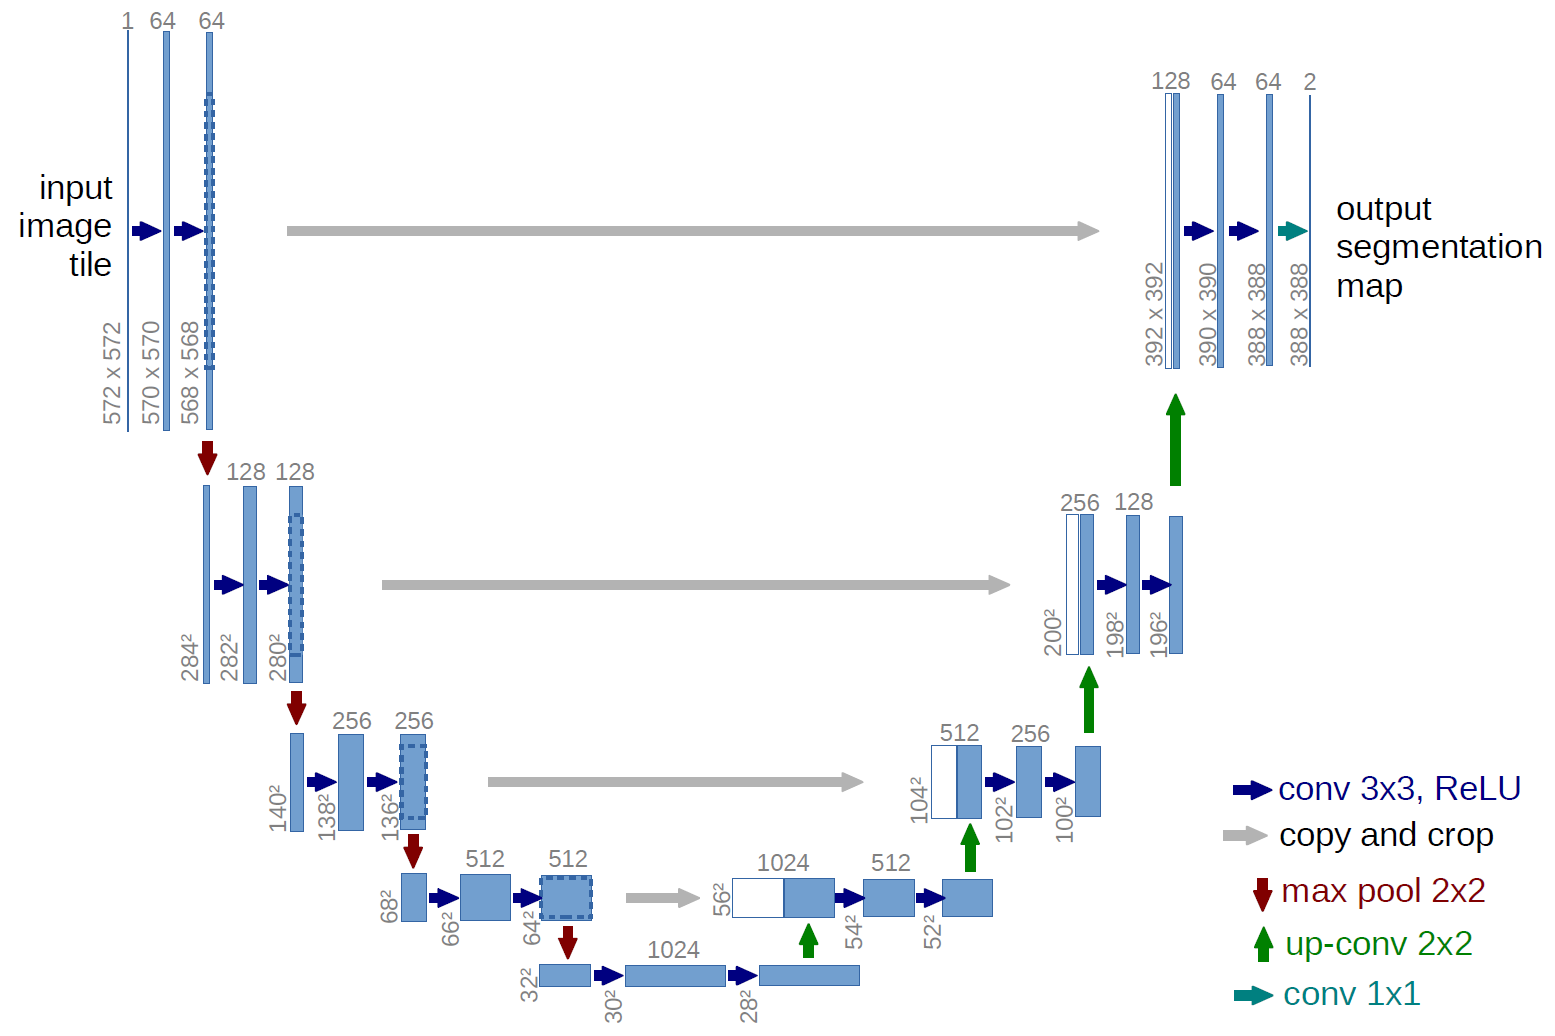
\includegraphics[width=0.95\textwidth]{u-net-architecture.png}
    \caption{U-Net架构示意图。编码器通过最大池化逐步降低空间分辨率并增加特征通道数；解码器通过转置卷积恢复空间分辨率；跳跃连接将编码器特征与解码器特征拼接，保留细节信息。}
    \label{fig:unet_arch}
\end{figure}

\textbf{编码器（Encoder）}：采用卷积层与最大池化交替的结构，每个阶段包含两个$3{\times}3$卷积（ReLU激活）和一个$2{\times}2$最大池化（步长为2）。特征通道数从64开始逐层翻倍（64→128→256→512），空间分辨率逐层减半（$572{\times}572$→$286{\times}286$→$143{\times}143$→$71{\times}71$）。

\textbf{瓶颈层（Bottleneck）}：编码器最后阶段之后是两个$3{\times}3$卷积层，特征通道数达到1024，空间分辨率降至$32{\times}32$。

\textbf{解码器（Decoder）}：采用转置卷积进行上采样，每个阶段包含一个$2{\times}2$转置卷积（步长为2）和两个$3{\times}3$卷积。跳跃连接将编码器对应阶段的特征图裁剪后与解码器上采样特征拼接，有效融合高层语义信息与低层细节信息。

\textbf{输出层}：最后通过$1{\times}1$卷积将特征映射到目标类别数，产生分割掩码。

参考基线的U-Net采用EfficientNet-B2作为编码器，而非原始U-Net的简单卷积结构。EfficientNet-B2通过复合缩放策略优化网络深度、宽度和分辨率，在ImageNet上预训练后迁移到医学图像分割任务，能够提取更具判别力的特征表示。

\subsubsection{前向传播流程}

算法~\ref{alg:unet_forward}描述了U-Net的前向传播过程。

\begin{algorithm}[H]
    \caption{U-Net前向传播}
    \label{alg:unet_forward}
    \KwIn{输入图像 $\bm{I} \in \mathbb{R}^{1 \times H \times W}$}
    \KwOut{分割概率图 $\hat{\bm{Y}} \in \mathbb{R}^{K \times H \times W}$}
    \tcp{编码阶段}
    \For{$i \leftarrow 1$ \KwTo $L$}{
        $\bm{e}_i \leftarrow \mrm{ConvBlock}(\bm{e}_{i-1})$ \tcp*{两个$3{\times}3$卷积 + ReLU}
        $\bm{s}_i \leftarrow \bm{e}_i$ \tcp*{保存跳跃连接特征}
        $\bm{e}_i \leftarrow \mrm{MaxPool}_{2\times2}(\bm{e}_i)$ \tcp*{空间分辨率减半}
    }
    $\bm{b} \leftarrow \mrm{ConvBlock}(\bm{e}_L)$ \tcp*{瓶颈层}
    \tcp{解码阶段}
    \For{$i \leftarrow L$ \KwTo $1$}{
        $\bm{d}_i \leftarrow \mrm{ConvTranspose}_{2\times2}(\bm{d}_{i+1})$ \tcp*{上采样，分辨率翻倍}
        $\bm{d}_i \leftarrow \mrm{Concat}(\bm{s}_i, \bm{d}_i)$ \tcp*{跳跃连接拼接}
        $\bm{d}_i \leftarrow \mrm{ConvBlock}(\bm{d}_i)$ \tcp*{特征融合}
    }
    $\hat{\bm{Y}} \leftarrow \mrm{Sigmoid}(\mrm{Conv}_{1\times1}(\bm{d}_1))$ \tcp*{输出分割概率}
\end{algorithm}

其中$\mrm{ConvBlock}$表示两个$3{\times}3$卷积层与ReLU激活函数的组合，$L=4$为编码器深度，$K=3$为目标类别数。跳跃连接通过拼接操作将编码器特征$\bm{s}_i$与解码器特征$\bm{d}_i$融合，使解码器同时获取高层语义信息与低层空间细节。

\subsection{Swin-UNETR v2架构}
\label{sec:arch}

本研究采用Swin-UNETR~v2作为基线分割网络，其整体架构如图~\ref{fig:swin_unetr_arch}所示。该架构创新性地将Swin Transformer编码器与U-Net风格解码器相结合，既保留了Transformer的全局上下文建模能力，又具备CNN解码器的精确空间定位能力。

\begin{figure}[H]
    \centering
    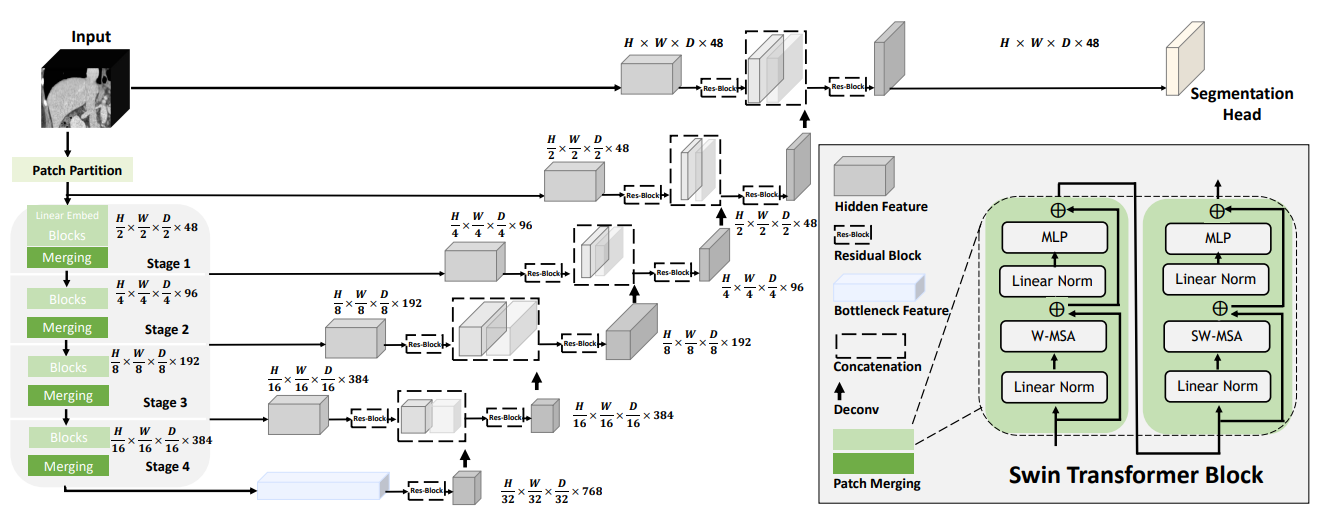
\includegraphics[width=0.98\textwidth]{swin_unetr.png}
    \caption{Swin-UNETR v2架构示意图。左侧为编码器的四个Stage，每个Stage包含Swin Transformer Block和Patch Merging操作；右侧展示了Swin Transformer Block的内部结构，包含W-MSA（窗口多头自注意力）和SW-MSA（移位窗口多头自注意力）两种注意力机制。解码器通过转置卷积上采样并与编码器特征进行跳跃连接融合。}
    \label{fig:swin_unetr_arch}
\end{figure}

\subsubsection{Patch Partition与线性嵌入}

输入图像首先经过Patch Partition操作，将$H{\times}W{\times}C$的图像划分为$N$个不重叠的patch（$N=(H{\times}W)/P^2$，其中$P$为patch大小）。每个patch通过线性投影层转换为固定维度的特征向量，形成初始特征序列：
\begin{equation}
    \bm{x}_0 = \mrm{Linear}(\text{flatten}(\text{PatchPartition}(I)))
\end{equation}
本研究中输入尺寸为$256{\times}256{\times}1$，patch大小为$4{\times}4$，因此初始特征维度为$64{\times}64{\times}48$。

\subsubsection{Swin Transformer编码器}

Swin Transformer编码器~\cite{liu2021swin}通过层级式特征提取与局部窗口自注意力机制，在保持线性计算复杂度的同时捕获多尺度全局特征。与ViT~\cite{dosovitskiy2021vit}采用全局自注意力不同，Swin Transformer借鉴了卷积网络的层级设计思想，通过移位窗口机制实现了线性复杂度的注意力计算。如图~\ref{fig:swin_unetr_arch}所示，编码器包含四个Stage，每个Stage由多个Swin Transformer Block和一个Patch Merging操作组成。

每个Swin Transformer Block包含两个连续的注意力模块：
\begin{align}
    \hat{\bm{z}}^{l} &= \mrm{W\text{-}MSA}\!\left(\mrm{LN}\!\left(\bm{z}^{l-1}\right)\right) + \bm{z}^{l-1}, \\
    \bm{z}^{l} &= \mrm{MLP}\!\left(\mrm{LN}\!\left(\hat{\bm{z}}^{l}\right)\right) + \hat{\bm{z}}^{l}, \\
    \hat{\bm{z}}^{l+1} &= \mrm{SW\text{-}MSA}\!\left(\mrm{LN}\!\left(\bm{z}^{l}\right)\right) + \bm{z}^{l}, \\
    \bm{z}^{l+1} &= \mrm{MLP}\!\left(\mrm{LN}\!\left(\hat{\bm{z}}^{l+1}\right)\right) + \hat{\bm{z}}^{l+1},
\end{align}

\textbf{W-MSA（Window Multi-Head Self-Attention）}：在固定大小的局部窗口内计算自注意力，注意力复杂度为$\mathcal{O}(N \cdot M^2 \cdot C)$，其中$M$为窗口大小。当$M \ll \sqrt{N}$时，复杂度近似线性于序列长度。

\textbf{SW-MSA（Shifted Window Multi-Head Self-Attention）}：通过循环移位操作改变窗口划分方式，使得相邻窗口中的patch能够进行信息交互，有效消除窗口边界带来的信息割裂问题。

\textbf{Patch Merging}：在相邻Stage之间进行特征降采样，通过拼接相邻patch并进行线性投影，将特征维度翻倍同时空间分辨率减半。编码器各Stage的特征维度与空间分辨率如表~\ref{tab:swin_stages}所示。

\begin{table}[H]
    \centering
    \caption{Swin-UNETR v2编码器各Stage特征维度与空间分辨率}
    \label{tab:swin_stages}
    \begin{tabular}{@{}llll@{}}
        \toprule
        \textbf{Stage} & \textbf{特征维度} & \textbf{空间分辨率} & \textbf{Patch大小} \\
        \midrule
        输入 & $1{\times}256{\times}256$ & $256{\times}256$ & $1{\times}1$ \\
        Stage 1 & $48{\times}128{\times}128$ & $128{\times}128$ & $4{\times}4$ \\
        Stage 2 & $96{\times}64{\times}64$ & $64{\times}64$ & $8{\times}8$ \\
        Stage 3 & $192{\times}32{\times}32$ & $32{\times}32$ & $16{\times}16$ \\
        Stage 4 & $384{\times}16{\times}16$ & $16{\times}16$ & $32{\times}32$ \\
        \bottomrule
    \end{tabular}
\end{table}

\subsubsection{CNN解码器}

解码器采用转置卷积逐步上采样特征图，并通过跳跃连接将编码器Stage 1-3的特征与解码器对应层级特征拼接（Concatenation）。每个解码器层级包含：
1. $2{\times}2$转置卷积，步长为2，将空间分辨率翻倍
2. 与编码器对应层级特征拼接
3. 两个$3{\times}3$卷积层进行特征融合

这种设计确保了高层语义信息与低层细节信息的有效融合，提升分割边界的精确定位能力。

\subsubsection{前向传播流程}

算法~\ref{alg:swin_unetr_forward}描述了Swin-UNETR v2的完整前向传播过程。

\begin{algorithm}[H]
    \caption{Swin-UNETR v2前向传播}
    \label{alg:swin_unetr_forward}
    \KwIn{输入图像 $\bm{I} \in \mathbb{R}^{1 \times H \times W}$}
    \KwOut{分割概率图 $\hat{\bm{Y}} \in \mathbb{R}^{K \times H \times W}$}
    \tcp{Patch Partition与线性嵌入}
    $\bm{x}_0 \leftarrow \mrm{Linear}(\mrm{PatchPartition}(\bm{I}, P{=}4))$ \tcp*{$\bm{x}_0 \in \mathbb{R}^{48 \times \frac{H}{4} \times \frac{W}{4}}$}
    \tcp{编码阶段}
    \For{$s \leftarrow 1$ \KwTo $4$}{
        \For{$b \leftarrow 1$ \KwTo $N_b^{(s)}$}{
            $\bm{x}_s \leftarrow \mrm{SwinBlock}(\bm{x}_s, \mrm{mode}{=}\text{W-MSA})$\;
            $\bm{x}_s \leftarrow \mrm{SwinBlock}(\bm{x}_s, \mrm{mode}{=}\text{SW-MSA})$\;
        }
        $\bm{f}_s \leftarrow \bm{x}_s$ \tcp*{保存跳跃连接特征}
        \If{$s < 4$}{
            $\bm{x}_{s+1} \leftarrow \mrm{PatchMerging}(\bm{x}_s)$ \tcp*{空间分辨率减半，通道数翻倍}
        }
    }
    \tcp{解码阶段}
    $\bm{d}_4 \leftarrow \bm{x}_4$ \tcp*{瓶颈特征}
    \For{$s \leftarrow 3$ \KwTo $1$}{
        $\bm{d}_s \leftarrow \mrm{ConvTranspose}_{2\times2}(\bm{d}_{s+1})$ \tcp*{上采样}
        $\bm{d}_s \leftarrow \mrm{Concat}(\bm{f}_s, \bm{d}_s)$ \tcp*{跳跃连接拼接}
        $\bm{d}_s \leftarrow \mrm{ConvBlock}(\bm{d}_s)$ \tcp*{特征融合}
    }
    $\hat{\bm{Y}} \leftarrow \mrm{Sigmoid}(\mrm{Conv}_{1\times1}(\bm{d}_1))$ \tcp*{输出分割概率}
\end{algorithm}

\subsubsection{窗口自注意力计算}

算法~\ref{alg:window_attn}详细描述了W-MSA与SW-MSA的计算过程。

\begin{algorithm}[H]
    \caption{窗口多头自注意力（W-MSA / SW-MSA）}
    \label{alg:window_attn}
    \KwIn{输入特征 $\bm{x} \in \mathbb{R}^{C \times H' \times W'}$，窗口大小 $M$，模式 $\mrm{mode} \in \{\text{W-MSA}, \text{SW-MSA}\}$，注意力头数 $h$}
    \KwOut{输出特征 $\bm{z} \in \mathbb{R}^{C \times H' \times W'}$}
    $\bm{z}^{(0)} \leftarrow \mrm{LN}(\bm{x})$\;
    \eIf{$\mrm{mode} = \text{SW-MSA}$}{
        $\bm{z}^{(0)} \leftarrow \mrm{CyclicShift}(\bm{z}^{(0)}, \lfloor M/2 \rfloor)$ \tcp*{循环移位}
    }{
        $\bm{z}^{(0)} \leftarrow \bm{z}^{(0)}$ \tcp*{无移位}
    }
    将 $\bm{z}^{(0)}$ 划分为 $\frac{H'W'}{M^2}$ 个 $M{\times}M$ 窗口 $\{\bm{w}_k\}$\;
    \For{每个窗口 $\bm{w}_k$}{
        $\bm{Q}_k, \bm{K}_k, \bm{V}_k \leftarrow \mrm{Linear}(\bm{w}_k)$ \tcp*{线性投影，各$C/h$维}
        $\bm{A}_k \leftarrow \mrm{Softmax}\!\left(\frac{\bm{Q}_k \bm{K}_k^\top}{\sqrt{C/h}} + \bm{B}\right)$ \tcp*{$\bm{B}$为相对位置偏置}
        $\bm{w}'_k \leftarrow \bm{A}_k \bm{V}_k$ \tcp*{注意力加权求和}
    }
    $\bm{z}^{(1)} \leftarrow \mrm{MergeWindows}(\{\bm{w}'_k\})$\;
    \eIf{$\mrm{mode} = \text{SW-MSA}$}{
        $\bm{z}^{(1)} \leftarrow \mrm{CyclicShift}(\bm{z}^{(1)}, -\lfloor M/2 \rfloor)$ \tcp*{反向循环移位}
    }{
        $\bm{z}^{(1)} \leftarrow \bm{z}^{(1)}$\;
    }
    $\bm{z} \leftarrow \mrm{MLP}(\mrm{LN}(\bm{z}^{(1)})) + \bm{z}^{(1)}$ \tcp*{残差连接 + MLP}
\end{algorithm}

其中相对位置偏置$\bm{B} \in \mathbb{R}^{M^2 \times M^2}$通过可学习参数索引获取，为每个注意力头提供独立的位置编码。SW-MSA通过循环移位使窗口边界处的patch能够与相邻窗口交互，有效扩大了感受野。

\subsubsection{网络配置}

表~\ref{tab:network_params}列出了本研究所使用的网络参数配置。

\begin{table}[H]
    \centering
    \caption{Swin-UNETR v2网络配置}
    \label{tab:network_params}
    \begin{tabular}{@{}ll@{}}
        \toprule
        \textbf{参数} & \textbf{值} \\
        \midrule
        输入通道数 & 1（灰度CT） \\
        输出通道数 & 3（肺、心脏、气管） \\
        特征维度 & 48 \\
        空间维度 & 2D \\
        梯度检查点 & 启用（节省显存） \\
        架构版本 & v2 \\
        窗口大小 & $7{\times}7$ \\
        注意力头数 & $\{3, 6, 12, 24\}$（各Stage） \\
        \bottomrule
    \end{tabular}
\end{table}

\subsection{基于UNet++的对比模型}
\label{sec:unetpp}

为系统评估不同架构在胸部CT多器官分割任务上的性能差异，本研究引入UNet++~\cite{zhou2018unetpp}作为对比模型。UNet++采用嵌套的U-Net架构，其核心结构如图~\ref{fig:unetpp_arch}所示。通过密集的跳跃连接路径，UNet++能够有效弥合编码器与解码器之间的语义鸿沟。

\begin{figure}[H]
    \centering
    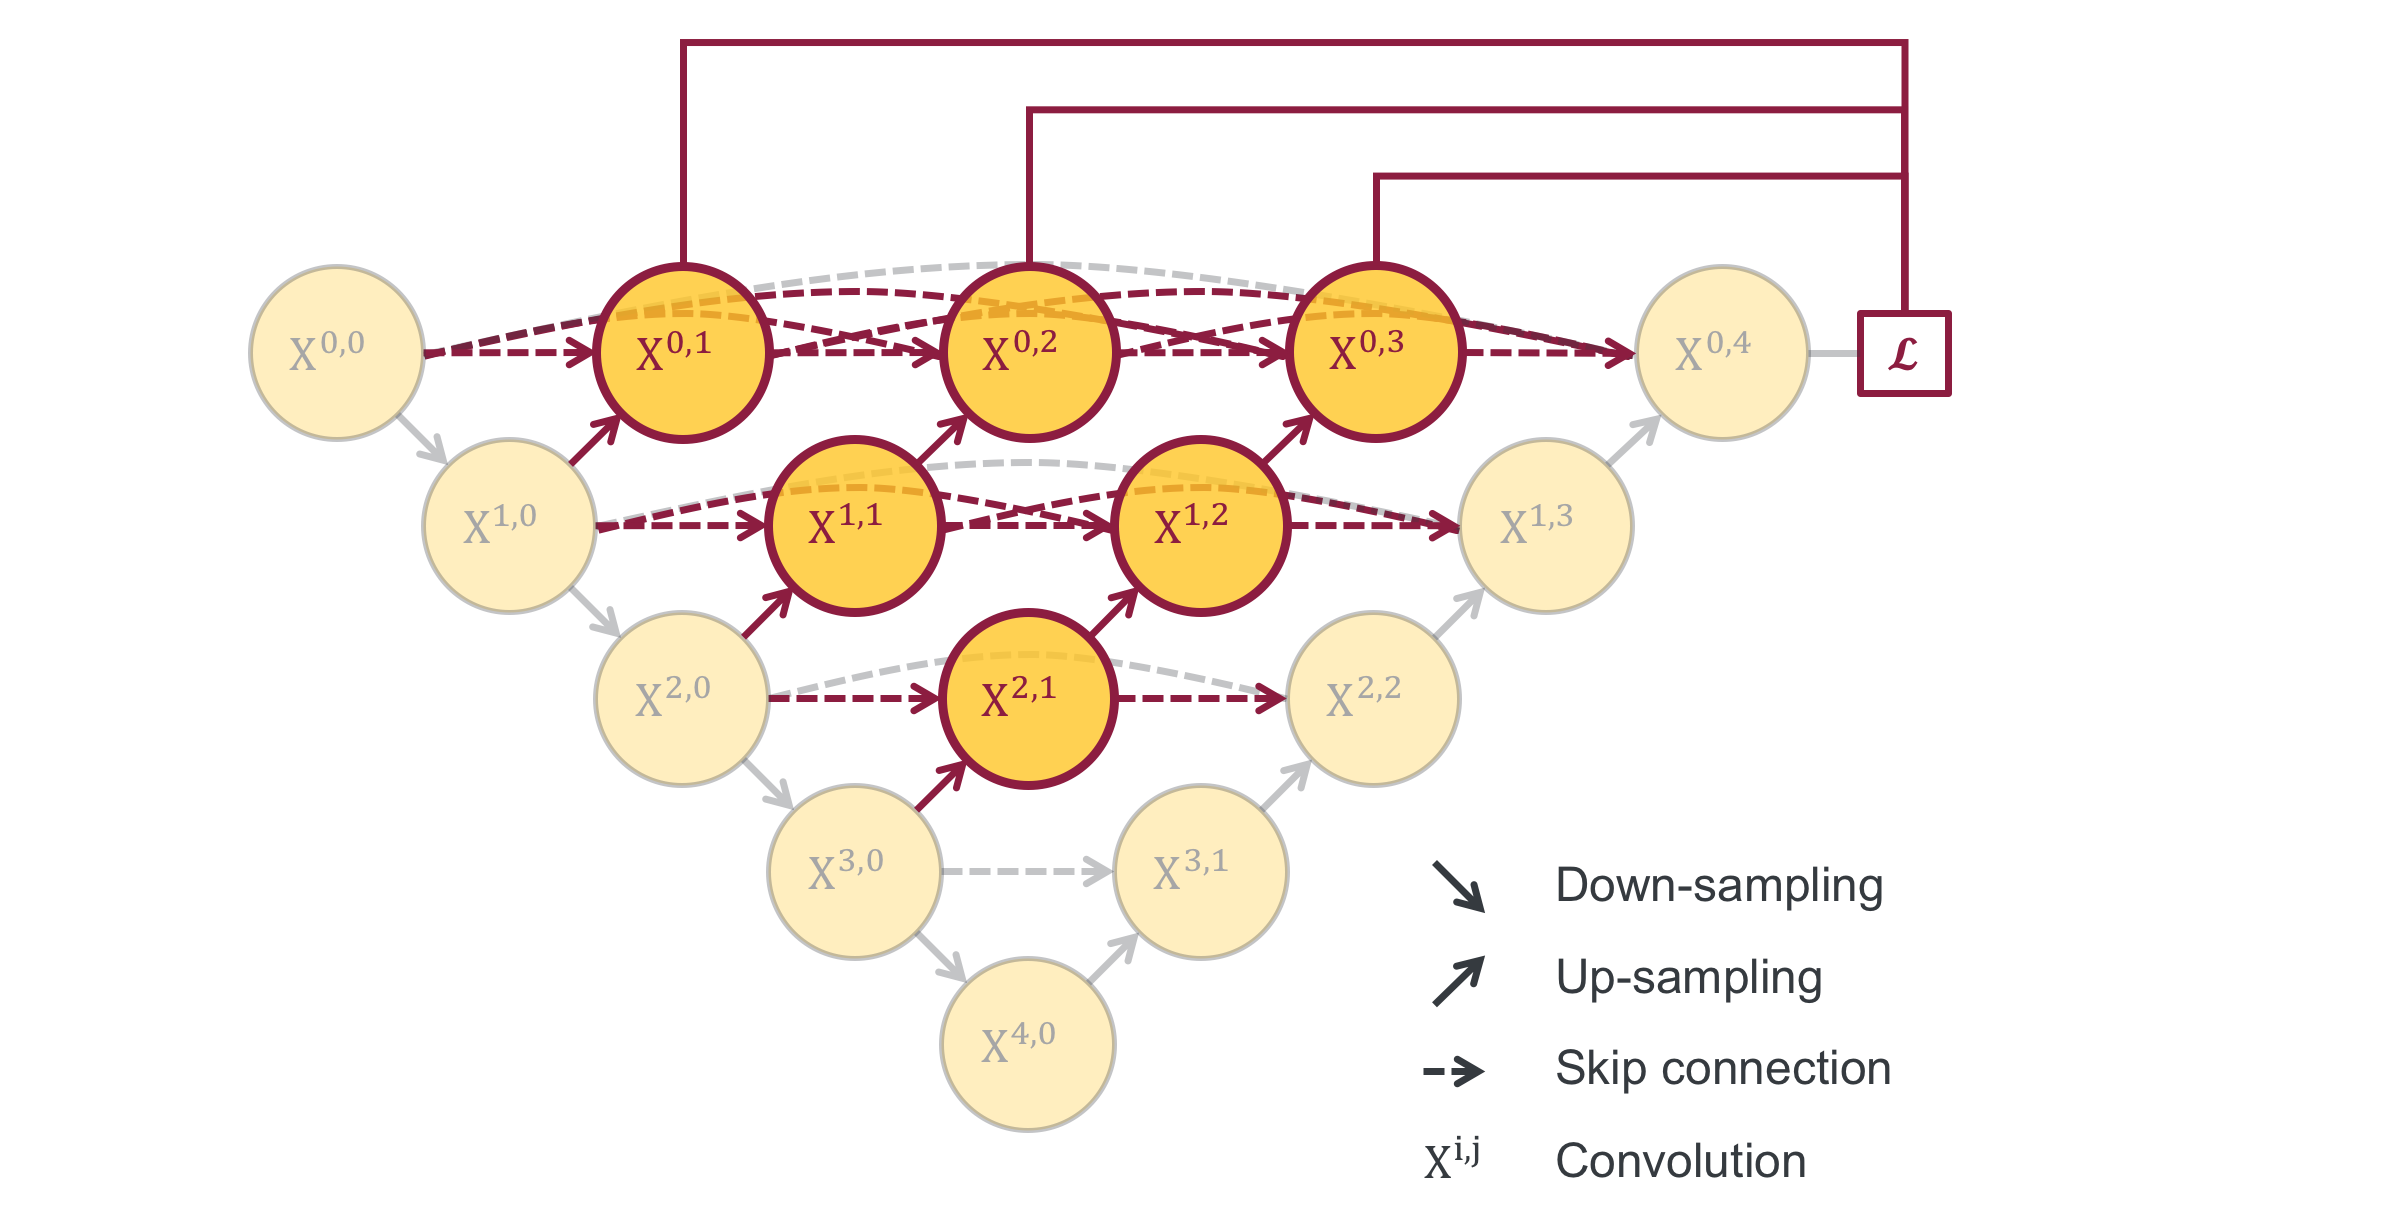
\includegraphics[width=0.85\textwidth]{fig_unet++.png}
    \caption{UNet++架构示意图。图中$X_{i,j}$表示第$i$层第$j$个卷积块。虚线表示跳跃连接，实线表示降采样/上采样路径。UNet++通过在编码器与解码器之间引入密集卷积块（橙色节点），逐步缩小语义差距。}
    \label{fig:unetpp_arch}
\end{figure}

\subsubsection{架构设计原理}

UNet++的核心创新在于其嵌套跳跃连接设计。传统U-Net的跳跃连接直接连接编码器第$i$层与解码器第$i$层，而UNet++在这两层之间引入了额外的卷积块，形成渐进式特征融合路径。具体来说，对于第$i$层第$j$个特征图$X_{i,j}$，其计算方式为：

\begin{equation}
    X_{i,j} = 
    \begin{cases} 
    \mrm{Conv}(X_{i-1,j}), & j=0 \\
    \mrm{Conv}\left(\mrm{Concat}\left(X_{i,j-1}, \mrm{Upsample}(X_{i+1,j-1}), X_{i-1,j}\right)\right), & j>0 
    \end{cases}
\end{equation}

其中$\mrm{Conv}$表示卷积操作，$\mrm{Concat}$表示特征拼接，$\mrm{Upsample}$表示上采样操作。

\subsubsection{EfficientNet-B2编码器}

UNet++的编码器采用EfficientNet-B2~\cite{tan2019efficientnet}作为骨干网络，并加载ImageNet预训练权重。EfficientNet通过复合缩放策略统一调整网络深度、宽度和输入分辨率：

\begin{align}
    \text{深度} &= \alpha^\phi \\
    \text{宽度} &= \beta^\phi \\
    \text{分辨率} &= \gamma^\phi
\end{align}

其中$\alpha \cdot \beta^2 \cdot \gamma^2 \approx 2$，$\phi$为缩放系数。B2变体（$\phi=1.1$）在精度与计算量之间取得了良好的平衡。

相较于Swin-UNETR~v2从头训练的Swin Transformer编码器，预训练的EfficientNet-B2编码器具有两方面优势：（1）ImageNet预训练提供了丰富的低层与中层视觉特征先验，有助于加速收敛并提升特征质量；（2）卷积架构的局部归纳偏置更适合医学图像中纹理与边界特征的提取。

\subsubsection{嵌套跳跃路径解码器}

UNet++的解码器采用嵌套跳跃连接（Nested Skip Pathways）设计，具有以下特点：

\textbf{渐进式特征融合}：通过在跳跃连接路径上添加卷积块，逐步将编码器的高层语义特征与解码器的低层细节特征融合，避免直接拼接带来的语义鸿沟。该设计受DenseNet~\cite{huang2017densely}密集连接思想的启发，通过特征重用提升信息流动效率。

\textbf{密集连接模式}：每个特征图$X_{i,j}$不仅连接到$X_{i,j-1}$和$X_{i-1,j}$，还通过上采样连接到$X_{i+1,j-1}$，形成密集的特征交互网络。

\textbf{深度监督}：UNet++在多个层级输出分割结果，通过深度监督（Deep Supervision）~\cite{lee2015deeply}策略联合优化，提升梯度流动和训练稳定性。

\subsubsection{前向传播流程}

算法~\ref{alg:unetpp_forward}描述了UNet++的前向传播过程，重点展示嵌套跳跃路径的计算逻辑。

\begin{algorithm}[H]
    \caption{UNet++前向传播}
    \label{alg:unetpp_forward}
    \KwIn{输入图像 $\bm{I} \in \mathbb{R}^{1 \times H \times W}$}
    \KwOut{分割概率图 $\hat{\bm{Y}} \in \mathbb{R}^{K \times H \times W}$}
    \tcp{编码器前向传播}
    \For{$i \leftarrow 0$ \KwTo $L$}{
        $X_{i,0} \leftarrow \mrm{EncBlock}_i(\bm{I})$ \tcp*{EfficientNet-B2编码器各阶段特征}
    }
    \tcp{嵌套跳跃路径}
    \For{$j \leftarrow 1$ \KwTo $L$}{
        \For{$i \leftarrow L-j$ \KwTo $0$ \textbf{step} $-1$}{
            $\bm{u} \leftarrow \mrm{Upsample}(X_{i+1,j-1})$ \tcp*{上采样深层特征}
            $\bm{c} \leftarrow \mrm{Concat}(X_{i,j-1}, \bm{u}, X_{i-1,j})$ \tcp*{密集拼接}
            $X_{i,j} \leftarrow \mrm{ConvBlock}(\bm{c})$ \tcp*{卷积融合}
        }
    }
    \tcp{深度监督（训练时）}
    \If{training}{
        \For{$i \leftarrow 0$ \KwTo $L-1$}{
            $\hat{\bm{Y}}_i \leftarrow \mrm{Sigmoid}(\mrm{Conv}_{1\times1}(X_{0,i}))$ \tcp*{各层输出}
        }
        $\mathcal{L} \leftarrow \sum_{i=0}^{L-1} w_i \cdot \mrm{Loss}(\hat{\bm{Y}}_i, \bm{Y})$ \tcp*{加权损失}
    }
    $\hat{\bm{Y}} \leftarrow \mrm{Sigmoid}(\mrm{Conv}_{1\times1}(X_{0,L}))$ \tcp*{最终输出}
\end{algorithm}

其中$L=4$为网络深度，$w_i$为各层损失的权重系数。深度监督策略在训练时同时优化多个层级的输出，使梯度能够更有效地回传至浅层网络，缓解深层网络的梯度消失问题。推理时仅使用最终输出$X_{0,L}$。

\subsubsection{网络配置}

表~\ref{tab:unetpp_params}列出了UNet++的网络参数配置。

\begin{table}[H]
    \centering
    \caption{UNet++网络配置}
    \label{tab:unetpp_params}
    \begin{tabular}{@{}ll@{}}
        \toprule
        \textbf{参数} & \textbf{值} \\
        \midrule
        编码器 & EfficientNet-B2 \\
        编码器权重 & ImageNet预训练 \\
        输入通道数 & 1（灰度CT） \\
        输出通道数 & 3（肺、心脏、气管） \\
        激活函数 & None（DiceFocalLoss内置Sigmoid） \\
        深度监督 & 启用 \\
        嵌套深度 & 4 \\
        \bottomrule
    \end{tabular}
\end{table}

\subsubsection{与U-Net的关键差异}

表~\ref{tab:unet_vs_unetpp}对比了标准U-Net与UNet++的核心差异：

\begin{table}[H]
    \centering
    \caption{U-Net与UNet++核心差异对比}
    \label{tab:unet_vs_unetpp}
    \begin{tabular}{@{}ll@{}}
        \toprule
        \textbf{特性} & \textbf{U-Net} \\
        \midrule
        跳跃连接方式 & 直接连接编码器与解码器 \\
        语义差距处理 & 无，直接拼接 \\
        特征融合深度 & 单层 \\
        深度监督 & 无 \\
        网络复杂度 & 较低 \\
        \midrule
        \textbf{特性} & \textbf{UNet++} \\
        \midrule
        跳跃连接方式 & 嵌套跳跃路径 \\
        语义差距处理 & 渐进式融合 \\
        特征融合深度 & 多层密集连接 \\
        深度监督 & 启用 \\
        网络复杂度 & 较高 \\
        \bottomrule
    \end{tabular}
\end{table}

\subsection{架构对比}
\label{sec:arch_compare}

表~\ref{tab:arch_compare}对参考基线与两种架构的核心设计差异进行了系统对比。

\begin{table}[H]
    \centering
    \caption{参考基线、Swin-UNETR v2与UNet++架构对比}
    \label{tab:arch_compare}
    \begin{adjustbox}{max width=\textwidth}
    \begin{tabular}{@{}lccc@{}}
        \toprule
        \textbf{特性} & \textbf{参考基线 (U-Net)} & \textbf{Swin-UNETR v2} & \textbf{UNet++ (EfficientNet-B2)} \\
        \midrule
        编码器类型 & EfficientNet-B2 (CNN) & Swin Transformer & EfficientNet-B2 (CNN) \\
        编码器预训练 & ImageNet预训练 & 无（从头训练） & ImageNet预训练 \\
        解码器类型 & CNN + 跳跃连接 & CNN + 跳跃连接 & 嵌套跳跃路径 \\
        特征提取范式 & 局部卷积 + 复合缩放 & 全局自注意力 & 局部卷积 + 复合缩放 \\
        归纳偏置 & 强（卷积局部性先验） & 弱（需数据驱动学习） & 强（卷积局部性先验） \\
        输出激活 & Sigmoid & 内置于损失函数 & 内置于损失函数 \\
        \bottomrule
    \end{tabular}
    \end{adjustbox}
\end{table}

三种架构的核心差异在于编码器的设计哲学：参考基线与UNet++均采用预训练的EfficientNet-B2编码器，卷积架构的局部归纳偏置与ImageNet预训练权重为其提供了良好的特征初始化；Swin-UNETR~v2采用Swin Transformer编码器，通过移位窗口自注意力机制捕获全局上下文信息，但缺乏局部归纳偏置，需要更多训练数据与更长训练周期来学习视觉特征。参考基线与UNet++的关键差异在于解码器设计：参考基线采用标准U-Net的直接跳跃连接，而UNet++采用嵌套跳跃路径，逐步缩小编码器与解码器特征之间的语义差距，理论上应有利于边界分割精度的提升。

\subsection{数据预处理}
\label{sec:preprocess}

数据预处理流程基于MONAI框架~\cite{cardoso2022monai}构建（参考基线基于albumentations框架），训练时与推理时的变换组合如表~\ref{tab:transforms}所示。由于三种架构的特性差异，参考基线、Swin-UNETR~v2与UNet++采用了不同强度的数据增强策略。

\begin{table}[H]
    \centering
    \caption{数据预处理与数据增强流程}
    \label{tab:transforms}
    \begin{adjustbox}{max width=\textwidth}
    \begin{tabular}{@{}llcccc@{}}
        \toprule
        \textbf{变换方法} & \textbf{参数} & \textbf{参考基线} & \textbf{Swin-UNETR训练} & \textbf{UNet++训练} & \textbf{推理} \\
        \midrule
        LoadImaged & keys=\{image, label\} & --- & \checkmark & \checkmark & \checkmark \\
        EnsureChannelFirstd & keys=\{image, label\} & --- & \checkmark & \checkmark & \checkmark \\
        ScaleIntensityd & keys=\{image\} & --- & \checkmark & \checkmark & \checkmark \\
        VerticalFlip & p=0.5 & \checkmark & --- & --- & --- \\
        Normalize & ImageNet mean/std & \checkmark & --- & --- & --- \\
        RandFlipd & prob=0.5, axis=\{0,1\} & --- & \checkmark & \checkmark & --- \\
        RandAffined & rotate, translate, scale & --- & \checkmark & \checkmark & --- \\
        RandRotate90d & prob=0.5 & --- & \checkmark & --- & --- \\
        RandGaussianNoised & prob=0.15, std=0.02 & --- & \checkmark & --- & --- \\
        RandAdjustContrastd & prob=0.15, $\gamma\in[0.8,1.2]$ & --- & \checkmark & --- & --- \\
        Resized & $256{\times}256$, bilinear/nearest & \checkmark & \checkmark & \checkmark & \checkmark \\
        ToTensord & keys=\{image, label\} & --- & \checkmark & \checkmark & \checkmark \\
        \bottomrule
    \end{tabular}
    \end{adjustbox}
\end{table}

参考基线采用最轻量的数据增强策略，仅使用VerticalFlip（p=0.5）与ImageNet归一化，这与其预训练编码器的良好特征初始化相匹配。

Swin-UNETR~v2采用了更重的数据增强策略，包含两类变换：（1）\textbf{空间变换}（RandFlipd、RandAffined、RandRotate90d），通过几何变换增强模型对器官位置与形态变化的鲁棒性；（2）\textbf{强度变换}（RandGaussianNoised、RandAdjustContrastd），通过模拟噪声与对比度差异增强模型对不同扫描条件的适应性。较重的数据增强旨在弥补Transformer编码器缺乏局部归纳偏置的不足，通过增加训练样本的多样性来提升模型的泛化能力。

UNet++采用了更轻量的数据增强策略，仅保留RandFlipd与RandAffined（概率降至0.3，变换范围缩小），去除了RandRotate90d、RandGaussianNoised和RandAdjustContrastd。这一设计基于以下考量：（1）EfficientNet-B2的ImageNet预训练权重已提供良好的特征初始化，无需通过强数据增强来弥补归纳偏置的不足；（2）更轻量的数据增强有助于模型更快地学习训练数据的分布特征，加速收敛；（3）较大的批大小（64）本身提供了更稳定的梯度估计，部分替代了数据增强的正则化效果。

输入图像统一缩放至$256{\times}256$，以满足Swin Transformer对输入尺寸为32倍数的要求，同时与EfficientNet-B2的输入分辨率保持一致。

\subsection{损失函数}
\label{sec:loss}

本研究采用DiceFocalLoss作为训练损失函数，该函数为Dice Loss~\cite{milletari2016v}与Focal Loss~\cite{lin2017focal}的加权组合：
\begin{equation}
    \mathcal{L} = \lambda_{\Dice} \cdot \mathcal{L}_{\Dice} + \lambda_{\Focal} \cdot \mathcal{L}_{\Focal}
    \label{eq:loss}
\end{equation}
其中，Dice Loss定义为：
\begin{equation}
    \mathcal{L}_{\Dice} = 1 - \frac{2\sum_{i}(p_i \cdot g_i) + \epsilon}{\sum_{i}p_i + \sum_{i}g_i + \epsilon}
    \label{eq:dice_loss}
\end{equation}
Focal Loss定义为：
\begin{equation}
    \mathcal{L}_{\Focal} = -\alpha_t (1 - p_t)^{\gamma} \log(p_t)
    \label{eq:focal_loss}
\end{equation}
式中$p_i$和$g_i$分别为预测概率与真实标签像素值，$\epsilon$为平滑因子，$\alpha_t$为类别权重，$\gamma$为聚焦参数。

Dice Loss直接优化分割重叠度，对类别不平衡具有天然鲁棒性；Focal Loss通过降低易分类样本的损失权重，使模型聚焦于难分类区域（如器官边界与小器官）。MONAI框架中DiceFocalLoss默认设置$\lambda_{\Dice}=\lambda_{\Focal}=1.0$，$\gamma=2.0$，并启用Sigmoid激活与背景通道包含。

\subsubsection{损失函数计算流程}

算法~\ref{alg:dice_focal_loss}描述了DiceFocalLoss的完整计算过程。

\begin{algorithm}[H]
    \caption{DiceFocalLoss计算}
    \label{alg:dice_focal_loss}
    \KwIn{模型输出 $\hat{\bm{Y}} \in \mathbb{R}^{K \times H \times W}$，真实标签 $\bm{Y} \in \{0,1\}^{K \times H \times W}$，权重 $\lambda_{\Dice}, \lambda_{\Focal}$，聚焦参数 $\gamma$}
    \KwOut{标量损失值 $\mathcal{L}$}
    \tcp{Sigmoid激活}
    $\bm{p} \leftarrow \mrm{Sigmoid}(\hat{\bm{Y}})$ \tcp*{预测概率}
    $\bm{p} \leftarrow \mrm{Clip}(\bm{p}, \epsilon, 1-\epsilon)$ \tcp*{数值稳定性裁剪}
    \tcp{Dice Loss计算}
    $\mrm{TP} \leftarrow \sum_{i} \bm{p}_i \cdot \bm{Y}_i$ \tcp*{逐通道真阳性}
    $\mrm{FP} \leftarrow \sum_{i} \bm{p}_i \cdot (1 - \bm{Y}_i)$ \tcp*{逐通道假阳性}
    $\mrm{FN} \leftarrow \sum_{i} (1 - \bm{p}_i) \cdot \bm{Y}_i$ \tcp*{逐通道假阴性}
    $\mathcal{L}_{\Dice} \leftarrow 1 - \frac{2 \cdot \mrm{TP} + \epsilon}{2 \cdot \mrm{TP} + \mrm{FP} + \mrm{FN} + \epsilon}$ \tcp*{逐通道Dice Loss}
    $\mathcal{L}_{\Dice} \leftarrow \mrm{Mean}_c(\mathcal{L}_{\Dice})$ \tcp*{通道平均}
    \tcp{Focal Loss计算}
    $\bm{p}_t \leftarrow \bm{Y} \cdot \bm{p} + (1 - \bm{Y}) \cdot (1 - \bm{p})$ \tcp*{正确分类概率}
    $\alpha_t \leftarrow \bm{Y} \cdot \alpha + (1 - \bm{Y}) \cdot (1 - \alpha)$ \tcp*{类别权重}
    $\mathcal{L}_{\Focal} \leftarrow -\alpha_t \cdot (1 - \bm{p}_t)^{\gamma} \cdot \log(\bm{p}_t)$ \tcp*{逐像素Focal Loss}
    $\mathcal{L}_{\Focal} \leftarrow \mrm{Mean}(\mathcal{L}_{\Focal})$ \tcp*{全局平均}
    \tcp{加权组合}
    $\mathcal{L} \leftarrow \lambda_{\Dice} \cdot \mathcal{L}_{\Dice} + \lambda_{\Focal} \cdot \mathcal{L}_{\Focal}$\;
\end{algorithm}

DiceFocalLoss的设计动机在于：Dice Loss通过直接优化重叠度指标，对前景与背景比例悬殊的类别（如气管）具有天然的鲁棒性；Focal Loss通过调制因子$(1-p_t)^\gamma$降低易分类样本的损失贡献，使模型在训练过程中聚焦于难分类区域。两者的组合实现了分割质量与训练稳定性的平衡。

\subsection{优化与训练}
\label{sec:optim}

模型训练采用AdamW优化器~\cite{loshchilov2017decoupled}，其将权重衰减与梯度更新解耦，相比标准Adam~\cite{kingma2015adam}具有更优的正则化效果。学习率调度采用余弦退火策略（Cosine Annealing）~\cite{smith2017cyclical}：
\begin{equation}
    \eta_t = \eta_{\min} + \frac{1}{2}(\eta_{\max} - \eta_{\min})\left(1 + \cos\frac{t\pi}{T_{\max}}\right)
    \label{eq:cosine}
\end{equation}
其中$\eta_{\max}=1{\times}10^{-4}$，$\eta_{\min}=1{\times}10^{-6}$。Swin-UNETR~v2设置$T_{\max}=200$，UNet++设置$T_{\max}=150$。该策略在训练初期以较大学习率快速收敛，后期以极小学习率精细调整，有效缓解Transformer架构对学习率敏感导致的训练震荡问题。完整训练流程如算法~\ref{alg:train}所示。

\begin{algorithm}[H]
    \caption{统一训练流程}
    \label{alg:train}
    \KwHyper{Epochs $T$, batch size $B$, seed $s{=}520$, model type $M$}
    \KwIn{Dataset $\mathcal{D}$}
    \KwOut{Trained model parameters $\theta^*$}
    设置随机种子 $s$\;
    \eIf{$M = $ Swin-UNETR v2}{
        初始化模型 $\theta$（随机），$T{\leftarrow}200$，$B{\leftarrow}16$\;
        配置重数据增强（含RandRotate90d、RandGaussianNoised等）\;
    }{
        初始化模型 $\theta$（EfficientNet-B2加载ImageNet预训练权重），$T{\leftarrow}150$，$B{\leftarrow}64$\;
        配置轻数据增强（仅RandFlipd、RandAffined）\;
    }
    初始化 AdamW 优化器、CosineAnnealingLR 调度器\;
    \For{$t \leftarrow 1$ \KwTo $T$}{
        从 $\mathcal{D}$ 中采样 mini-batch $\{(\bm{x}_i, \bm{y}_i)\}_{i=1}^{B}$\;
        预处理：$\bm{y}_i \leftarrow \bm{y}_i[:, [2,1,0], :, :]$ \tcp*{BGR $\to$ RGB}
        前向传播：$\hat{\bm{y}}_i \leftarrow f_\theta(\bm{x}_i)$\;
        计算损失：$\mathcal{L} = \mrm{DiceFocalLoss}(\hat{\bm{y}}_i, \bm{y}_i)$\;
        反向传播：$\theta \leftarrow \theta - \eta_t \cdot \nabla_\theta \mathcal{L}$\;
        更新学习率：通过 CosineAnnealingLR 更新 $\eta_t$\;
        \If{$t \bmod 10 = 0$}{
            保存 checkpoint：$f_{\theta}^{(t)}$\;
        }
    }
\end{algorithm}

% ============================================================
\section{实验设置}
\label{sec:setup}
% ============================================================

\subsection{数据集}
\label{sec:dataset}

本研究使用Kaggle平台公开的Chest CT Segmentation数据集\footnote{\url{https://www.kaggle.com/datasets/polomarco/chest-ct-segmentation}}，包含胸部CT横断面图像及对应的三器官分割掩码。数据集统计信息如表~\ref{tab:dataset}所示。

\begin{table}[H]
    \centering
    \caption{数据集统计信息}
    \label{tab:dataset}
    \begin{tabular}{@{}ll@{}}
        \toprule
        \textbf{项} & \textbf{描述} \\
        \midrule
        图像-掩码对总数 & 1,000 \\
        训练集 & 800（80\,\%） \\
        验证集 & 200（20\,\%） \\
        图像格式 & JPG, $512{\times}512$ \\
        掩码格式 & JPG（RGB）, 阈值 $\geq 240$ \\
        分割类别 & 肺（R通道）、心脏（G通道）、气管（B通道） \\
        配对关系 & \texttt{train.csv}: ImageId $\leftrightarrow$ MaskId \\
        \bottomrule
    \end{tabular}
\end{table}

掩码为RGB三通道图像，像素值$\geq 240$的区域为有效分割区域。原始数据集通道顺序为BGR（OpenCV格式），训练与测试代码中通过通道交换操作\texttt{labels[:, [2,1,0], :, :]}将其转换为RGB顺序，对应[肺、心脏、气管]。

\subsection{环境配置}
\label{sec:env}

本实验的硬件与软件环境如表~\ref{tab:env}所示。

\begin{table}[H]
    \centering
    \caption{实验环境配置}
    \label{tab:env}
    \begin{tabular}{@{}ll@{}}
        \toprule
        \textbf{类别} & \textbf{配置} \\
        \midrule
        操作系统 & Linux \\
        GPU & NVIDIA A100 \\
        PyTorch & $\geq 2.0$ \\
        MONAI & $\geq 1.5.2$ \\
        其他依赖 & Pandas, NumPy, scikit-learn, Matplotlib, tqdm \\
        \bottomrule
    \end{tabular}
\end{table}

\subsubsection{训练配置}

表~\ref{tab:train_config}汇总了两种架构的完整训练配置。

\begin{table}[H]
    \centering
    \caption{训练配置对比}
    \label{tab:train_config}
    \begin{adjustbox}{max width=\textwidth}
    \begin{tabular}{@{}lccc@{}}
        \toprule
        \textbf{超参数} & \textbf{参考基线} & \textbf{Swin-UNETR v2} & \textbf{UNet++} \\
        \midrule
        架构 & U-Net (EfficientNet-B2) & Swin-UNETR v2 & UNet++ (EfficientNet-B2) \\
        编码器预训练 & ImageNet & 无（从头训练） & ImageNet \\
        优化器 & Adam & AdamW \cite{loshchilov2017decoupled} & AdamW \cite{loshchilov2017decoupled} \\
        学习率 & $8{\times}10^{-5}$ & $1{\times}10^{-4}$ & $1{\times}10^{-4}$ \\
        权重衰减 & --- & $1{\times}10^{-5}$ & $1{\times}10^{-5}$ \\
        学习率调度 & ReduceLROnPlateau & CosineAnnealingLR & CosineAnnealingLR \\
        $T_{\max}$ / patience & patience=3 & $T_{\max}=200$ & $T_{\max}=150$ \\
        $\eta_{\min}$ & --- & $10^{-6}$ & $10^{-6}$ \\
        损失函数 & BCEDiceLoss & DiceFocalLoss & DiceFocalLoss \\
        批大小 & 8 & 16 & 64 \\
        训练轮数 & 100+ & 200 & 150 \\
        数据划分 & random\_state=69 & random\_state=520 & random\_state=520 \\
        随机种子 & 555 & 520 & 520 \\
        数据增强 & 轻增强（仅翻转+归一化） & 重增强（含旋转90°、噪声、对比度） & 轻增强（仅翻转、仿射） \\
        框架 & albumentations & MONAI & MONAI \\
        \bottomrule
    \end{tabular}
    \end{adjustbox}
\end{table}

参考基线与本研究后续实验在优化器、损失函数、学习率调度等方面均存在显著差异。本研究后续两组Swin-UNETR~v2实验与UNet++实验共享相同的优化器（AdamW）、损失函数（DiceFocalLoss）和学习率调度策略（CosineAnnealingLR），以确保对比的公平性。关键差异在于批大小与训练轮数：UNet++采用批大小64（Swin-UNETR~v2为16），训练150轮（Swin-UNETR~v2为200轮）。批大小的选择综合考虑了模型显存占用与梯度估计稳定性，UNet++的EfficientNet-B2编码器参数效率更高，允许使用更大的批大小。

\subsection{实验设计}
\label{sec:exp_design}

本研究共设计三组独立实验，以全面评估方法的有效性与参数优化的影响。实验配置的确定经历了以下方法学演进过程：

\textbf{第一阶段——参考基线}：项目初期首先复现了数据集提供方的开源U-Net实现（\texttt{exmaple.py}），该实现采用U-Net + EfficientNet-B2编码器，配合BCEDiceLoss与Adam优化器，在验证集上取得了val\_dice$\approx$0.968的性能。这一基线为后续实验建立了性能参考。

\textbf{第二阶段——Swin-UNETR v2初步探索}：基于参考基线的性能参考，本研究采用Swin-UNETR~v2作为主架构进行探索，初始配置为批大小64、无数据增强，仅训练10轮。该初步探索的结果显示性能有限，为后续配置优化提供了方向。

\textbf{第三阶段——配置优化}：基于初步探索的结果，对训练配置进行了系统性优化：（1）引入全面的数据增强策略（RandFlipd、RandAffined、RandGaussianNoised、RandAdjustContrastd、RandRotate90d），以弥补Transformer编码器缺乏局部归纳偏置的不足；（2）将批大小从64降至16，以提升泛化能力；（3）引入CosineAnnealingLR余弦退火学习率调度器，缓解训练震荡问题；（4）将Adam优化器替换为AdamW，实现解耦权重衰减正则化；（5）将BCEDiceLoss替换为DiceFocalLoss，通过Focal机制增强对难分类样本的学习。该优化配置构成了后续基准实验与参数优化实验的基础。

\textbf{第四阶段——架构对比}：在Swin-UNETR~v2优化配置的基础上，引入UNet++（EfficientNet-B2预训练编码器）作为对比架构，采用更轻量的数据增强策略和更大的批大小（64），充分利用预训练编码器的快速收敛特性。

基于上述方法学演进，本研究设计了以下三组独立实验：

\textbf{基于Swin-UNETR v2的基准实验}：采用优化后的Swin-UNETR~v2架构，训练200轮，批大小16，随机种子520，完整数据增强与余弦退火调度。该实验旨在建立Swin-UNETR~v2在胸部CT多器官分割任务上的基线性能。

\textbf{基于Swin-UNETR v2的参数优化实验}：采用与基准实验相同的Swin-UNETR~v2架构与超参数配置，训练200轮，批大小16，随机种子520。该实验旨在验证批大小从64降至16这一关键参数优化对模型泛化能力与收敛稳定性的影响。与基准实验相比，参数优化实验在训练后期表现出更稳定的收敛特性（mDSC仅从0.9390降至0.9371，而基准实验从0.9388降至0.9068），验证了小批大小对缓解过拟合的有效性。

\textbf{基于UNet++的对比实验}：采用UNet++（EfficientNet-B2编码器）架构，训练150轮，批大小64，随机种子520，轻量数据增强策略。该实验旨在通过对比不同架构的性能，评估CNN预训练编码器与嵌套跳跃路径设计相对于Transformer架构在分割精度上的差异。

基准实验与参数优化实验构成参数优化验证组，对比实验构成架构对比组。三组独立实验共享相同的数据集划分（random\_state=520）、损失函数（DiceFocalLoss）与优化器（AdamW）配置，确保对比的公平性与结论的可靠性。

\subsection{评价指标}
\label{sec:metrics}

本研究采用以下指标评估分割性能：

\textbf{Dice相似系数（Dice Similarity Coefficient, DSC）}：衡量预测与真实分割的重叠程度，取值范围为$[0, 1]$，值越大表示分割效果越好：
\begin{equation}
    \Dice = \frac{2|A \cap B|}{|A| + |B|}
    \label{eq:dice}
\end{equation}
其中$A$为预测分割区域，$B$为真实标注区域。

\textbf{交并比（Intersection over Union, IoU）}：又称Jaccard系数，衡量预测与真实分割的交并比：
\begin{equation}
    \IoU = \frac{|A \cap B|}{|A \cup B|}
    \label{eq:iou}
\end{equation}

\textbf{平均Dice/平均IoU（mDSC/mIoU）}：所有类别Dice/IoU的算术平均值，用于综合评估多类别分割性能。

% ============================================================
\section{实验结果与分析}
\label{sec:results}
% ============================================================

如第~\ref{sec:exp_design}节所述，本研究共进行三组独立实验：基准实验与参数优化实验采用Swin-UNETR~v2架构（相同配置，验证参数优化效果），对比实验采用UNet++架构（对比研究）。此外，参考基线（U-Net + EfficientNet-B2）的性能数据为实验结果提供了重要的参照。本节依次展示参考基线结果、各实验的定量结果、训练动态与对比分析。

\subsection{定量结果}
\label{sec:quantitative}

\subsubsection{参考基线结果}

表~\ref{tab:results_baseline}展示了参考基线（U-Net + EfficientNet-B2）在验证集上的最佳性能。该基线基于数据集提供方的开源实现，使用BCEDiceLoss与Adam优化器，在100轮预训练模型基础上继续训练。

\begin{table}[H]
    \centering
    \caption{参考基线最佳验证集性能（U-Net + EfficientNet-B2）}
    \label{tab:results_baseline}
    \begin{tabular}{@{}lcc@{}}
        \toprule
        \textbf{指标} & \textbf{最佳值} & \textbf{备注} \\
        \midrule
        val\_dice & $\approx$0.968 & 整体Dice系数（非逐器官） \\
        val\_jaccard & $\approx$0.949 & 整体IoU（非逐器官） \\
        \bottomrule
    \end{tabular}
\end{table}

需要指出的是，参考基线采用整体Dice/Jaccard系数作为评价指标，即对所有像素统一计算而不区分器官类别，而本研究后续实验采用逐器官计算Dice系数再取平均（mDSC）的评价方式。此外，基线使用不同的数据划分（random\_state=69）和训练框架（albumentations），因此其结果与本研究实验之间不宜直接进行数值比较，但可作为性能水平的参考。

\subsubsection{基于Swin-UNETR v2的基准实验关键轮次结果}

表~\ref{tab:results_exp1}展示了基准实验在关键训练轮次的定量评估结果。

\begin{table}[H]
    \centering
    \caption{基于Swin-UNETR v2的基准实验关键训练轮次定量评估结果}
    \label{tab:results_exp1}
    \small
    \begin{adjustbox}{max width=\textwidth}
    \begin{tabular}{@{}ccccc@{}}
        \toprule
        \textbf{轮次} & \textbf{DSC$_\text{肺}$} & \textbf{DSC$_\text{心脏}$} & \textbf{DSC$_\text{气管}$} & \textbf{mDSC} \\
        \midrule
        10 & 0.8308 & 0.8785 & 0.6852 & 0.7982 \\
        20 & 0.8766 & 0.9114 & 0.8306 & 0.8729 \\
        50 & 0.8895 & 0.9009 & 0.8722 & 0.8876 \\
        100 & 0.9065 & 0.8978 & 0.9327 & 0.9124 \\
        140 & 0.9372 & 0.8956 & 0.9436 & 0.9255 \\
        170 & 0.9612 & 0.9043 & 0.9458 & 0.9371 \\
        180 & \textbf{0.9632} & \textbf{0.9132} & \textbf{0.9398} & \textbf{0.9388} \\
        200 & 0.9622 & 0.8433 & 0.9148 & 0.9068 \\
        \bottomrule
    \end{tabular}
    \end{adjustbox}
\end{table}

基准实验的最优模型出现在第180轮，mDSC达0.9388。值得注意的是，第200轮时心脏DSC出现显著下降（从0.9132降至0.8433），导致mDSC降至0.9068，表明Swin-UNETR~v2在训练后期存在过拟合风险。

\subsubsection{基于Swin-UNETR v2的参数优化实验关键轮次结果}

表~\ref{tab:results_exp2}展示了参数优化实验在关键训练轮次的定量评估结果，该实验取得了Swin-UNETR~v2两组独立实验中的最佳性能。

\begin{table}[H]
    \centering
    \caption{基于Swin-UNETR v2的参数优化实验关键训练轮次定量评估结果}
    \label{tab:results_exp2}
    \small
    \begin{adjustbox}{max width=\textwidth}
    \begin{tabular}{@{}ccccccccc@{}}
        \toprule
        \textbf{轮次} & \textbf{DSC$_\text{肺}$} & \textbf{IoU$_\text{肺}$} & \textbf{DSC$_\text{心脏}$} & \textbf{IoU$_\text{心脏}$} & \textbf{DSC$_\text{气管}$} & \textbf{IoU$_\text{气管}$} & \textbf{mDSC} & \textbf{mIoU} \\
        \midrule
        10 & 0.8148 & 0.7888 & 0.6385 & 0.6202 & 0.5224 & 0.4873 & 0.6586 & 0.6321 \\
        20 & 0.8512 & 0.8275 & 0.8094 & 0.7924 & 0.6139 & 0.5822 & 0.7581 & 0.7340 \\
        50 & 0.8313 & 0.8057 & 0.7383 & 0.7209 & 0.8629 & 0.8331 & 0.8109 & 0.7865 \\
        100 & 0.9113 & 0.8905 & 0.8351 & 0.8199 & 0.9225 & 0.8959 & 0.8896 & 0.8688 \\
        150 & 0.9621 & 0.9420 & 0.8936 & 0.8799 & 0.9412 & 0.9183 & 0.9323 & 0.9134 \\
        170 & 0.9650 & 0.9461 & 0.8958 & 0.8823 & 0.9449 & 0.9231 & 0.9352 & 0.9172 \\
        180 & 0.9652 & 0.9464 & 0.9018 & 0.8883 & 0.9451 & 0.9234 & 0.9374 & 0.9194 \\
        190 & \textbf{0.9660} & \textbf{0.9475} & \textbf{0.9054} & \textbf{0.8920} & \textbf{0.9458} & \textbf{0.9243} & \textbf{0.9390} & \textbf{0.9212} \\
        200 & 0.9664 & 0.9480 & 0.8995 & 0.8860 & 0.9455 & 0.9242 & 0.9371 & 0.9194 \\
        \bottomrule
    \end{tabular}
    \end{adjustbox}
\end{table}

参数优化实验的最优模型出现在第190轮，mDSC达0.9390。与基准实验相比，参数优化实验在训练后期（第200轮）的性能下降幅度较小（mDSC从0.9390降至0.9371，仅下降0.0019），而基准实验从0.9388降至0.9068（下降0.0320），表明批大小从64降至16这一参数优化有效缓解了训练后期的过拟合问题，提升了模型的泛化稳定性。

\subsubsection{基于UNet++的对比实验关键轮次结果}

表~\ref{tab:results_exp3}展示了对比实验在关键训练轮次的定量评估结果。

\begin{table}[H]
    \centering
    \caption{基于UNet++的对比实验关键训练轮次定量评估结果}
    \label{tab:results_exp3}
    \small
    \begin{adjustbox}{max width=\textwidth}
    \begin{tabular}{@{}ccccc@{}}
        \toprule
        \textbf{轮次} & \textbf{DSC$_\text{肺}$} & \textbf{DSC$_\text{心脏}$} & \textbf{DSC$_\text{气管}$} & \textbf{mDSC} \\
        \midrule
        10 & 0.8846 & 0.8765 & 0.7427 & 0.8346 \\
        20 & 0.9366 & 0.8694 & 0.8520 & 0.8860 \\
        50 & 0.9470 & 0.9173 & 0.9008 & 0.9217 \\
        60 & 0.9568 & 0.9617 & 0.9319 & 0.9501 \\
        100 & 0.9689 & 0.9701 & 0.9505 & 0.9632 \\
        120 & 0.9695 & 0.9703 & 0.9544 & 0.9647 \\
        140 & 0.9703 & 0.9712 & 0.9560 & 0.9658 \\
        150 & \textbf{0.9702} & \textbf{0.9718} & \textbf{0.9563} & \textbf{0.9661} \\
        \bottomrule
    \end{tabular}
    \end{adjustbox}
\end{table}

对比实验的最优模型出现在第150轮（最后一个训练轮次），mDSC达0.9661，显著优于Swin-UNETR~v2的两组独立实验。值得注意的是，UNet++仅用10轮训练即达到mDSC~0.8346，已接近Swin-UNETR~v2训练50轮的水平，充分体现了预训练编码器的优势。此外，UNet++在训练过程中未出现性能下降现象，模型在整个训练周期内保持稳定提升。

\subsubsection{最佳性能对比}

表~\ref{tab:best_results}汇总了参考基线与三组独立实验的最佳性能结果。

\begin{table}[H]
    \centering
    \caption{参考基线与三组独立实验最佳性能对比}
    \label{tab:best_results}
    \begin{adjustbox}{max width=\textwidth}
    \begin{tabular}{@{}lccccc@{}}
        \toprule
        \textbf{指标} & \textbf{参考基线} & \textbf{基准实验} & \textbf{参数优化实验} & \textbf{对比实验} & \textbf{整体最佳} \\
        & U-Net (EfficientNet-B2) & Swin-UNETR v2 & Swin-UNETR v2 & UNet++ & \\
        \midrule
        DSC$_\text{肺}$ & --- & 0.9632 & 0.9660 & \textbf{0.9702} & \textbf{0.9702} \\
        DSC$_\text{心脏}$ & --- & 0.9132 & 0.9054 & \textbf{0.9718} & \textbf{0.9718} \\
        DSC$_\text{气管}$ & --- & 0.9398 & 0.9458 & \textbf{0.9563} & \textbf{0.9563} \\
        mDSC & --- & 0.9388 & 0.9390 & \textbf{0.9661} & \textbf{0.9661} \\
        val\_dice & $\approx$0.968 & --- & --- & --- & $\approx$0.968 \\
        \textbf{最佳轮次} & 100+ & 180 & 190 & 150 & - \\
        \bottomrule
    \end{tabular}
    \end{adjustbox}
\end{table}

注：参考基线采用整体Dice系数（不区分器官类别），而本研究实验采用逐器官DSC及mDSC，两者评价方式不同，因此基线的逐器官DSC以"---"标注，不宜直接数值对比。

从表中可以得出以下关键发现：（1）UNet++在所有器官类别上均显著优于Swin-UNETR~v2，mDSC提升2.71个百分点；（2）UNet++的心脏分割性能提升最为显著（DSC从0.9132提升至0.9718，提升5.86个百分点），表明预训练编码器对心脏这类边界模糊器官的分割具有明显优势；（3）基准实验与参数优化实验的Swin-UNETR~v2结果非常接近（mDSC差异仅0.0002），但参数优化实验在训练后期稳定性显著更优，验证了批大小优化对缓解过拟合的有效性；（4）参考基线的整体val\_dice$\approx$0.968与UNet++的mDSC=0.9661处于相近水平，但需注意两者评价方式与数据划分不同。

\subsection{训练动态}
\label{sec:dynamics}

\subsubsection{损失收敛分析}

图~\ref{fig:loss_all}展示了三组独立实验的训练损失变化趋势。

\begin{figure}[H]
    \centering
    \begin{tikzpicture}
    \begin{groupplot}[
        group style={
            group size=1 by 3,
            vertical sep=2.0cm,
        },
        width=0.82\textwidth,
        height=4.2cm,
        scale only axis,
        grid=major,
        grid style={dashed, gray!15},
        tick label style={font=\footnotesize},
        label style={font=\small},
        title style={font=\small\bfseries},
    ]
    % --- Exp1 Loss ---
    \nextgroupplot[
        ylabel={训练损失},
        title={(a) 基准实验（Swin-UNETR v2）},
        xmin=0, xmax=200,
        ymin=0.25, ymax=1.0,
    ]
    \addplot[cBlue, thick, mark=none, smooth] coordinates {
        (1,0.9239) (5,0.7518) (10,0.6848) (20,0.5611) (25,0.5551)
        (30,0.5515) (40,0.5467) (50,0.5438) (60,0.5430) (70,0.4078)
        (80,0.3929) (90,0.3949) (100,0.3833) (110,0.3815) (120,0.3864)
        (125,0.3804) (130,0.3907) (140,0.3746) (150,0.3924) (160,0.3811)
        (162,0.3197) (170,0.2984) (180,0.3060) (190,0.3112) (200,0.2996)
    };

    % --- Exp2 Loss ---
    \nextgroupplot[
        ylabel={训练损失},
        title={(b) 参数优化实验（Swin-UNETR v2）},
        xmin=0, xmax=200,
        ymin=0.25, ymax=1.0,
        xticklabels={},
    ]
    \addplot[cRed, thick, mark=none, smooth] coordinates {
        (1,0.8599) (5,0.6461) (10,0.5993) (20,0.5791) (25,0.5101)
        (30,0.4399) (40,0.4517) (50,0.4705) (60,0.4266) (70,0.4053)
        (80,0.4039) (90,0.4026) (100,0.4017) (110,0.3985) (120,0.3920)
        (125,0.3814) (130,0.3305) (140,0.3136) (150,0.3104) (160,0.3069)
        (170,0.3056) (180,0.3044) (190,0.3034) (200,0.3037)
    };

    % --- Exp3 Loss ---
    \nextgroupplot[
        ylabel={训练损失},
        xlabel={训练轮次（Epoch）},
        title={(c) 对比实验（UNet++）},
        xmin=0, xmax=150,
        ymin=0, ymax=1.0,
    ]
    \addplot[cGreen, thick, mark=none, smooth] coordinates {
        (1,0.9617) (5,0.7130) (10,0.5921) (20,0.5647) (30,0.5575)
        (40,0.5538) (50,0.5506) (51,0.4445) (60,0.0664) (70,0.0504)
        (80,0.0459) (90,0.0434) (100,0.0396) (110,0.0371) (120,0.0363)
        (130,0.0345) (140,0.0343) (150,0.0336)
    };

    \end{groupplot}
    \end{tikzpicture}
    \caption{三组独立实验的训练损失曲线。(a)(b) Swin-UNETR~v2呈现两阶段收敛特征，损失从$\sim$0.9降至$\sim$0.30；(c) UNet++在第50-60轮间出现急剧下降（从0.55降至0.07），最终收敛至0.034，远低于Swin-UNETR~v2。}
    \label{fig:loss_all}
\end{figure}

三组独立实验的损失曲线呈现出截然不同的收敛特征：

\textbf{Swin-UNETR~v2基准与参数优化实验}：损失曲线呈现两阶段收敛特征。第一阶段（第1-125轮）损失快速下降，从初始的$\sim$0.9降至$\sim$0.38；第二阶段（第126-200轮）损失在较低水平缓慢收敛，最终稳定在0.30左右。基准实验在第162轮附近出现一次显著的损失跳变（从0.38降至0.32），可能归因于余弦退火调度器在训练中期学习率仍较大时，模型参数跨越损失曲面鞍点所致。

\textbf{UNet++对比实验}：损失曲线呈现出更为独特的三阶段收敛特征。第一阶段（第1-50轮）损失缓慢下降，从0.96降至0.55，与Swin-UNETR~v2的收敛速度相近；第二阶段（第51-60轮）损失急剧下降，从0.44骤降至0.07，这一突变可能与预训练编码器的特征激活有关——当学习率降至特定阈值时，预训练特征与任务特定特征实现有效对齐，导致损失骤降；第三阶段（第60-150轮）损失在极低水平缓慢收敛，最终稳定在0.034左右，远低于Swin-UNETR~v2的0.30，表明UNet++在训练集上实现了更充分的拟合。

\subsubsection{各器官Dice系数变化趋势}

图~\ref{fig:dice_all}展示了三组独立实验中各器官Dice系数随训练轮次的变化趋势。

\begin{figure}[H]
    \centering
    \begin{tikzpicture}
    \begin{groupplot}[
        group style={
            group size=1 by 3,
            vertical sep=2.0cm,
        },
        width=0.82\textwidth,
        height=4.2cm,
        scale only axis,
        grid=major,
        grid style={dashed, gray!15},
        tick label style={font=\footnotesize},
        label style={font=\small},
        title style={font=\small\bfseries},
        ymin=0.45, ymax=1.0,
    ]
    % --- Exp1 Dice ---
    \nextgroupplot[
        ylabel={Dice相似系数},
        title={(a) 基准实验（Swin-UNETR v2）},
        xmin=0, xmax=200,
        xticklabels={},
        legend style={
            at={(0.98,0.45)}, anchor=east,
            font=\scriptsize, draw=gray!30,
            fill=white, fill opacity=0.9,
            rounded corners=1pt,
            row sep=1pt,
        },
    ]
    \addplot[cBlue, thick, mark=none, smooth] coordinates {
        (10,0.8308) (20,0.8766) (50,0.8895) (100,0.9065)
        (140,0.9372) (170,0.9612) (180,0.9632) (200,0.9622)
    };
    \addlegendentry{肺}
    \addplot[cRed, thick, mark=none, smooth] coordinates {
        (10,0.8785) (20,0.9114) (50,0.9009) (100,0.8978)
        (140,0.8956) (170,0.9043) (180,0.9132) (200,0.8433)
    };
    \addlegendentry{心脏}
    \addplot[cGreen, thick, mark=none, smooth] coordinates {
        (10,0.6852) (20,0.8306) (50,0.8722) (100,0.9327)
        (140,0.9436) (170,0.9458) (180,0.9398) (200,0.9148)
    };
    \addlegendentry{气管}

    % --- Exp2 Dice ---
    \nextgroupplot[
        ylabel={Dice相似系数},
        title={(b) 参数优化实验（Swin-UNETR v2）},
        xmin=0, xmax=200,
        xticklabels={},
        legend style={
            at={(0.98,0.45)}, anchor=east,
            font=\scriptsize, draw=gray!30,
            fill=white, fill opacity=0.9,
            rounded corners=1pt,
            row sep=1pt,
        },
    ]
    \addplot[cBlue, thick, mark=none, smooth] coordinates {
        (10,0.8148) (20,0.8512) (50,0.8313) (100,0.9113)
        (150,0.9621) (170,0.9650) (180,0.9652) (190,0.9660) (200,0.9664)
    };
    \addlegendentry{肺}
    \addplot[cRed, thick, mark=none, smooth] coordinates {
        (10,0.6385) (20,0.8094) (50,0.7383) (100,0.8351)
        (150,0.8936) (170,0.8958) (180,0.9018) (190,0.9054) (200,0.8995)
    };
    \addlegendentry{心脏}
    \addplot[cGreen, thick, mark=none, smooth] coordinates {
        (10,0.5224) (20,0.6139) (50,0.8629) (100,0.9225)
        (150,0.9412) (170,0.9449) (180,0.9451) (190,0.9458) (200,0.9455)
    };
    \addlegendentry{气管}

    % --- Exp3 Dice ---
    \nextgroupplot[
        ylabel={Dice相似系数},
        xlabel={训练轮次（Epoch）},
        title={(c) 对比实验（UNet++）},
        xmin=0, xmax=150,
        legend style={
            at={(0.98,0.45)}, anchor=east,
            font=\scriptsize, draw=gray!30,
            fill=white, fill opacity=0.9,
            rounded corners=1pt,
            row sep=1pt,
        },
    ]
    \addplot[cBlue, thick, mark=none, smooth] coordinates {
        (10,0.8846) (20,0.9366) (50,0.9470) (60,0.9568)
        (100,0.9689) (120,0.9695) (140,0.9703) (150,0.9702)
    };
    \addlegendentry{肺}
    \addplot[cRed, thick, mark=none, smooth] coordinates {
        (10,0.8765) (20,0.8694) (50,0.9173) (60,0.9617)
        (100,0.9701) (120,0.9703) (140,0.9712) (150,0.9718)
    };
    \addlegendentry{心脏}
    \addplot[cGreen, thick, mark=none, smooth] coordinates {
        (10,0.7427) (20,0.8520) (50,0.9008) (60,0.9319)
        (100,0.9505) (120,0.9544) (140,0.9560) (150,0.9563)
    };
    \addlegendentry{气管}

    \end{groupplot}
    \end{tikzpicture}
    \caption{三组独立实验各器官Dice系数变化趋势。(a)(b) Swin-UNETR~v2中肺收敛最快，心脏与气管后期波动明显；(c) UNet++中三类器官均在第60轮后快速收敛至0.95以上，心脏DSC甚至超过肺，展现出优异的分割性能。}
    \label{fig:dice_all}
\end{figure}

从图中可以观察到以下规律：

\textbf{Swin-UNETR~v2基准与参数优化实验}：肺DSC在训练早期即快速上升至0.90以上，后期稳定在0.96附近；心脏DSC上升较为缓慢，在第130轮后趋于0.90，但基准实验在第200轮出现显著下降（0.8433），表明存在过拟合风险；气管DSC在训练初期波动较大，最终稳定在0.94左右。

\textbf{UNet++对比实验}：三类器官的DSC均在第60轮后快速上升至0.95以上，展现出极为高效的收敛特性。特别值得注意的是，心脏DSC在第60轮出现跳变（从0.9173升至0.9617），与损失曲线的骤降点吻合，此后持续稳定提升至0.9718。UNet++中心脏DSC甚至超过了肺DSC，这在Swin-UNETR~v2的实验中从未观察到，表明预训练编码器对心脏分割的提升尤为显著。

\subsubsection{各实验最佳模型性能对比}

图~\ref{fig:bar_chart}以柱状图形式直观对比了三组独立实验最优模型在各器官上的DSC。

\begin{figure}[H]
    \centering
    \begin{tikzpicture}
    \begin{axis}[
        ybar,
        width=0.85\textwidth,
        height=6cm,
        scale only axis,
        bar width=10pt,
        xlabel={器官},
        ylabel={Dice相似系数（DSC）},
        ymin=0.86, ymax=1.0,
        symbolic x coords={肺, 心脏, 气管, mDSC},
        xtick=data,
        x tick label style={font=\small},
        tick label style={font=\footnotesize},
        label style={font=\small},
        legend style={
            at={(0.5,-0.20)}, anchor=north,
            legend columns=3,
            font=\footnotesize, draw=gray!30,
            fill=white, fill opacity=0.95,
            rounded corners=1pt,
            /tikz/every even column/.append style={column sep=12pt},
        },
        grid=major,
        grid style={dashed, gray!15},
        enlarge x limits=0.22,
        nodes near coords,
        every node near coord/.append style={
            font=\tiny,
            anchor=south,
            yshift=1pt,
        },
    ]
    \addplot[fill=cBlue!65, draw=cBlue!90] coordinates {
        (肺,0.9632) (心脏,0.9132) (气管,0.9398) (mDSC,0.9388)
    };
    \addlegendentry{基准实验 (Swin-UNETR v2)}

    \addplot[fill=cRed!55, draw=cRed!85] coordinates {
        (肺,0.9660) (心脏,0.9054) (气管,0.9458) (mDSC,0.9390)
    };
    \addlegendentry{参数优化实验 (Swin-UNETR v2)}

    \addplot[fill=cGreen!55, draw=cGreen!85] coordinates {
        (肺,0.9702) (心脏,0.9718) (气管,0.9563) (mDSC,0.9661)
    };
    \addlegendentry{对比实验 (UNet++)}

    \end{axis}
    \end{tikzpicture}
    \caption{三组独立实验最佳模型各器官DSC对比。UNet++在所有器官上均优于Swin-UNETR~v2，心脏分割提升最为显著（+5.86pp）。}
    \label{fig:bar_chart}
\end{figure}

\subsection{Swin-UNETR v2与UNet++对比分析}
\label{sec:compare}

基于上述实验结果，本节从多个维度对两种架构进行系统对比分析。

\subsubsection{分割精度对比}

UNet++在所有器官类别上均显著优于Swin-UNETR~v2。表~\ref{tab:improvement}量化了UNet++相对于Swin-UNETR~v2最佳结果的性能提升。

\begin{table}[H]
    \centering
    \caption{UNet++相对于Swin-UNETR~v2的性能提升}
    \label{tab:improvement}
    \begin{tabular}{@{}lccc@{}}
        \toprule
        \textbf{器官} & \textbf{Swin-UNETR v2最佳} & \textbf{UNet++最佳} & \textbf{提升} \\
        \midrule
        肺 & 0.9660 & 0.9702 & +0.42pp \\
        心脏 & 0.9132 & 0.9718 & +5.86pp \\
        气管 & 0.9458 & 0.9563 & +1.05pp \\
        mDSC & 0.9390 & 0.9661 & +2.71pp \\
        \bottomrule
    \end{tabular}
\end{table}

心脏分割的性能提升最为显著（+5.86pp），这一结果可从以下角度理解：心脏与周围纵隔组织的灰度差异较小，边界模糊，对特征提取的质量要求更高。Swin-UNETR~v2从头训练的Transformer编码器需要大量数据来学习有效的边界特征，而UNet++的预训练EfficientNet-B2编码器已具备丰富的边缘与纹理特征提取能力，能够更精确地定位心脏边界。

\subsubsection{收敛速度对比}

两种架构的收敛速度存在显著差异。以mDSC达到0.90为基准：Swin-UNETR~v2需要约100轮训练（参数优化实验第100轮mDSC=0.8896），而UNet++仅用约20轮即达到mDSC=0.8860，在第60轮已达到mDSC=0.9501。UNet++的收敛速度约为Swin-UNETR~v2的5倍，这主要归功于预训练编码器提供的良好特征初始化。

此外，UNet++的训练过程更为稳定，未出现Swin-UNETR~v2中观察到的后期性能下降现象。Swin-UNETR~v2基准实验在第200轮出现心脏DSC骤降（0.9132$\to$0.8433），而UNet++在整个训练周期内各器官DSC均保持单调递增或稳定，表现出更优的训练稳定性。

\subsubsection{训练效率对比}

从训练效率角度，UNet++仅需150轮训练即达到mDSC=0.9661，而Swin-UNETR~v2需要200轮训练仅达到mDSC=0.9390。结合批大小差异（UNet++批大小64 vs Swin-UNETR~v2批大小16），UNet++在每个epoch中处理更多的样本梯度，进一步加速了有效收敛。

\subsection{定性可视化}
\label{sec:qualitative}

图~\ref{fig:seg_vis}展示了典型样本的分割效果可视化。UNet++对比实验的模型在肺、心脏和气管三类器官上均取得了视觉上令人满意的分割结果，预测掩码与真实掩码高度吻合。

\begin{figure}[H]
    \centering
    \begin{subfigure}[b]{0.45\textwidth}
        \centering
        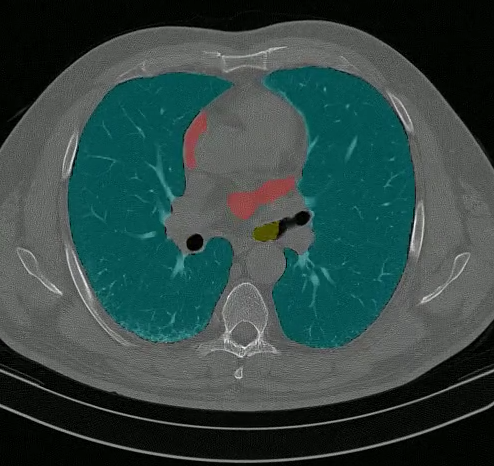
\includegraphics[width=\textwidth]{ground_truth.png}
        \caption{真实标注（Ground Truth）}
        \label{fig:seg_gt}
    \end{subfigure}
    \hfill
    \begin{subfigure}[b]{0.45\textwidth}
        \centering
        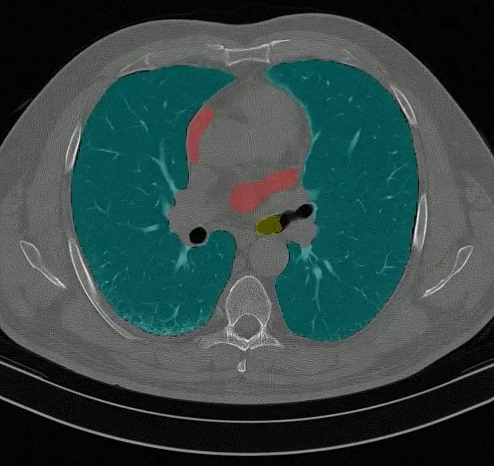
\includegraphics[width=\textwidth]{prediction.png}
        \caption{模型预测（Prediction）}
        \label{fig:seg_pred}
    \end{subfigure}
    
    \vspace{0.5cm}
    \begin{tikzpicture}[font=\footnotesize]
        \begin{scope}[shift={(0,0)}]
            \fill[cBlue!60] (0,0) rectangle (0.35,0.35);
            \draw[gray!50, line width=0.5pt] (0,0) rectangle (0.35,0.35);
            \node[right, font=\small] at (0.42,0.175) {肺（Lung）};
        \end{scope}
        \begin{scope}[shift={(4.2,0)}]
            \fill[cRed!60] (0,0) rectangle (0.35,0.35);
            \draw[gray!50, line width=0.5pt] (0,0) rectangle (0.35,0.35);
            \node[right, font=\small] at (0.42,0.175) {心脏（Heart）};
        \end{scope}
        \begin{scope}[shift={(8.4,0)}]
            \fill[cGreen!60] (0,0) rectangle (0.35,0.35);
            \draw[gray!50, line width=0.5pt] (0,0) rectangle (0.35,0.35);
            \node[right, font=\small] at (0.42,0.175) {气管（Trachea）};
        \end{scope}
    \end{tikzpicture}
    
    \caption{UNet++模型分割可视化结果。左图为真实标注，右图为模型预测。青色表示肺部区域，红色表示心脏区域，黄色表示气管区域。可以观察到模型在肺、心脏和气管的分割边界处与真实标注高度一致，尤其是心脏区域的边界定位非常精确。}
    \label{fig:seg_vis}
\end{figure}

从可视化结果可以看出：（1）肺部区域分割完整，左右肺叶均被准确识别；（2）心脏区域边界清晰，与周围纵隔组织区分明显；（3）气管结构被精确分割，即使在狭窄部位也保持良好的连续性。这表明UNet++模型能够有效捕获胸部CT图像中不同器官的形态特征，实现高精度的多器官分割。

% ============================================================
\section{讨论}
\label{sec:discussion}
% ============================================================

\subsection{Swin-UNETR v2与UNet++的对比分析}

本研究的实验结果清晰地表明，UNet++（EfficientNet-B2编码器）在胸部CT多器官分割任务上全面优于Swin-UNETR~v2。这一性能差异可从以下维度进行深入分析：

\textbf{1. 预训练编码器的关键作用}。Swin-UNETR~v2的Swin Transformer编码器从头训练，缺乏先验特征知识，需要通过大量训练数据与训练轮次来学习视觉特征。相比之下，UNet++的EfficientNet-B2编码器加载了ImageNet预训练权重，尽管ImageNet与医学CT图像的领域差异较大，但预训练权重仍提供了有价值的低层特征（如边缘、纹理检测）和中层特征（如形状组合），这些特征经微调后可有效地迁移至CT分割任务。这一发现与医学图像分割领域的已有研究一致：在有限数据集上，预训练编码器通常优于从头训练的编码器。

\textbf{2. 归纳偏置的影响}。卷积神经网络的局部归纳偏置（局部连接、权值共享、平移等变性）天然适合图像处理任务，尤其是对局部纹理与边界特征的提取。Swin Transformer虽然通过移位窗口机制实现了全局建模能力，但其弱归纳偏置意味着模型需要更多数据来学习这些局部特征。在仅800张训练图像的有限数据条件下，卷积架构的归纳偏置优势更为突出。

\textbf{3. 嵌套跳跃路径的语义桥接效应}。UNet++的嵌套跳跃连接通过逐步缩小编码器与解码器特征之间的语义差距，使传递至解码器的特征更具语义一致性。相比之下，Swin-UNETR~v2采用传统的直接跳跃连接，编码器浅层特征（低级纹理）与解码器深层特征（高级语义）之间的语义鸿沟可能影响分割边界的精确性。

\textbf{4. 批大小与数据增强的交互效应}。UNet++采用批大小64（Swin-UNETR~v2为16），更大的批大小提供了更稳定的梯度估计，有助于模型在预训练权重的良好初始化附近进行高效优化。同时，UNet++采用了更轻量的数据增强策略，避免了过度增强对预训练特征的破坏。这一组合（大批大小+轻增强+预训练权重）在有限数据集上表现出了优异的效果。

\textbf{5. 收敛稳定性的差异}。Swin-UNETR~v2在训练后期出现了性能下降现象（基准实验第200轮心脏DSC骤降），表明Transformer架构在长训练周期中存在过拟合风险。UNet++在整个训练过程中保持稳定提升，未出现性能回退，这得益于预训练权重的正则化效应与更大批大小带来的梯度稳定性。

\subsection{与参考基线的对比分析}

数据集提供方的开源U-Net实现（EfficientNet-B2编码器 + BCEDiceLoss）在验证集上取得了val\_dice$\approx$0.968的性能，这一结果为本研究提供了重要的参考基准。将本研究实验结果与参考基线进行对比分析：

\textbf{1. 性能水平对比}。参考基线的整体val\_dice$\approx$0.968与本研究UNet++的mDSC=0.9661处于相近水平。然而，需要指出的是，两者采用了不同的评价方式：基线采用整体Dice系数（对所有像素统一计算，不区分器官类别），而本研究采用逐器官DSC再取平均（mDSC）。整体Dice系数倾向于被占比最大的器官（肺）主导，而mDSC对每个器官赋予相同权重，因此小器官（气管）的性能对mDSC的影响更大。此外，两者使用了不同的数据划分（random\_state=69 vs 520），训练/验证集的样本构成存在差异，进一步限制了直接数值比较的有效性。

\textbf{2. 架构演进}。参考基线采用标准U-Net架构，本研究UNet++采用嵌套U-Net架构（UNet++），两者均使用EfficientNet-B2编码器。UNet++的嵌套跳跃连接设计通过逐步缩小编码器与解码器特征之间的语义差距，理论上应优于标准U-Net的直接跳跃连接。然而，由于评价方式与数据划分的差异，无法从当前实验结果中直接量化这一架构改进的贡献。

\textbf{3. 训练策略差异}。参考基线采用BCEDiceLoss + Adam + ReduceLROnPlateau的组合，而本研究采用DiceFocalLoss + AdamW + CosineAnnealingLR的组合。DiceFocalLoss通过Focal机制对难分类样本赋予更高权重，可能对小器官（气管）的分割更为有利；AdamW的解耦权重衰减提供了更优的正则化效果；CosineAnnealingLR的周期性退火策略有助于模型跳出局部最优。这些训练策略的差异也是本研究方法与参考基线之间的重要区别。

\textbf{4. 方法论启示}。参考基线与UNet++均采用预训练EfficientNet-B2编码器，且均取得了优异的分割性能，进一步验证了预训练编码器在有限数据条件下的关键作用。相比之下，从头训练的Swin-UNETR~v2（mDSC=0.9390）与预训练编码器架构之间存在明显差距，表明在胸部CT分割任务中，编码器的预训练策略比架构本身的选择（U-Net vs UNet++ vs Swin-UNETR）对最终性能的影响更为显著。

\subsection{器官分割难度分析}

综合三组独立实验的结果，器官分割难度呈现以下规律：

\textbf{肺}：在两种架构中均最易分割，DSC稳定在0.96以上。肺组织在CT图像中占比最大（约占图像面积的30-40\%）且对比度高（含气组织与周围软组织灰度差异显著），这些有利条件使得即使较简单的模型也能取得良好的分割效果。

\textbf{气管}：气管像素占比最小（<5\%），但得益于DiceFocalLoss对难分类样本的聚焦效应，两种架构均取得了较好的分割效果。Swin-UNETR~v2的气管DSC为0.9458，UNet++为0.9563，提升幅度（+1.05pp）相对较小，表明DiceFocalLoss已有效缓解了气管的类别不平衡问题。

\textbf{心脏}：心脏是两种架构性能差异最大的器官（Swin-UNETR~v2最佳0.9132 vs UNet++ 0.9718，提升5.86pp）。心脏分割困难的原因在于：（1）心脏与周围纵隔组织的灰度差异较小，边界模糊；（2）心脏形态存在较大的个体差异；（3）心脏区域的灰度值与背景较为接近。UNet++的预训练编码器提供了更精确的边界特征提取能力，嵌套跳跃连接改善了边界处的特征融合效果，这两者共同促成了心脏分割性能的显著提升。

\subsection{损失函数的有效性}

DiceFocalLoss在两种架构中均展现了良好的效果。Dice部分直接优化分割重叠度，对类别不平衡具有天然鲁棒性；Focal部分通过降低易分类样本的损失权重，使模型聚焦于难分类区域（如器官边界与小器官）。两者结合有效缓解了类别不平衡问题，使得气管这类小器官的DSC能够达到0.94以上。

\subsection{局限性分析}

本研究存在以下局限性：

1. \textbf{数据集规模有限}：本实验使用的Kaggle数据集仅有1,000对图像-掩码对，与医学图像分割领域常用的大规模数据集相比规模较小。更大规模、多中心的数据集将有助于进一步验证两种架构的性能差异，特别是Swin-UNETR~v2在更大数据集上是否能够缩小与UNet++的差距。

2. \textbf{仅为2D分割}：本研究采用的是2D分割方法，没有利用CT层间的连续性信息。3D分割方法可能能够利用更多的上下文信息，进一步提升分割精度。

3. \textbf{对比实验的变量控制}：对比实验（UNet++）与基准实验、参数优化实验（Swin-UNETR~v2）在批大小、训练轮数和数据增强策略上存在差异，这些混淆变量可能影响架构对比的结论。理想的对比实验应仅改变架构本身，控制其他变量不变。然而，不同架构的最优训练配置本身存在差异，完全控制变量可能无法反映各架构的实际潜力。

4. \textbf{缺乏更多方法的对比}：本研究仅对比了Swin-UNETR~v2与UNet++两种架构，未涉及TransUNet、nnU-Net等其他前沿方法，无法全面评估本方法在领域内的相对优势。

\subsection{未来工作展望}

基于本研究的结果和局限性，未来可以从以下方向进行探索：

1. \textbf{Swin-UNETR v2的预训练策略}：探索为Swin Transformer编码器引入自监督预训练（如Masked Image Modeling），以弥补其缺乏预训练权重的不足，评估预训练对Swin-UNETR~v2性能的提升幅度。

2. \textbf{3D分割方法}：将2D分割方法扩展为3D版本，充分利用CT图像的层间信息，探索3D上下文对分割性能的提升潜力。

3. \textbf{混合架构设计}：结合Transformer的全局建模能力与CNN的局部特征提取优势，设计混合编码器架构，如CNN提取局部特征后接Transformer建模全局依赖。

4. \textbf{模型轻量化与部署}：通过知识蒸馏、剪枝、量化等技术压缩模型，使其能够在资源受限的环境中部署。

5. \textbf{跨数据集泛化能力验证}：在多个公开数据集上评估本方法的性能，并探索域适应技术，提升模型在不同来源数据上的泛化能力。

% ============================================================
\section{结论}
\label{sec:conclusion}
% ============================================================

本研究针对胸部CT图像的多器官分割任务，系统比较了Swin-UNETR~v2与UNet++（EfficientNet-B2编码器）两种架构的性能，并以数据集提供方的开源U-Net实现作为参考基线。在Kaggle Chest CT Segmentation数据集上进行了三组独立实验：基准实验与参数优化实验采用Swin-UNETR~v2（相同配置，验证参数优化效果），对比实验采用UNet++（架构对比）。

实验结果表明：（1）Swin-UNETR~v2的基准实验与参数优化实验最佳mDSC分别为0.9388与0.9390，参数优化实验在训练后期表现出更稳定的收敛特性（mDSC仅下降0.0019 vs 基准实验下降0.0320），验证了批大小优化对缓解过拟合的有效性；（2）UNet++取得了0.9661的mDSC，显著优于Swin-UNETR~v2，其中肺、心脏、气管的DSC分别为0.9702、0.9718和0.9563；（3）UNet++的收敛速度约为Swin-UNETR~v2的5倍，且训练过程更为稳定，未出现后期性能下降现象；（4）参考基线（U-Net + EfficientNet-B2）的整体val\_dice$\approx$0.968，与UNet++的mDSC=0.9661处于相近水平，进一步验证了预训练编码器在有限数据条件下的关键作用。

性能差异的核心原因在于：预训练编码器提供了良好的特征初始化，卷积架构的局部归纳偏置更适合有限数据条件下的医学图像分割，嵌套跳跃连接有效改善了边界处的特征融合。这些发现为胸部CT分割任务的架构选择提供了重要参考：在训练数据有限的场景下，采用预训练编码器的CNN架构可能比从头训练的Transformer架构更为高效，且编码器的预训练策略比架构本身的选择对最终性能的影响更为显著。

本研究的贡献包括：（1）系统比较了Transformer与CNN预训练编码器架构在胸部CT分割任务上的性能差异；（2）揭示了预训练编码器、归纳偏置与数据增强策略对分割性能的交互影响；（3）通过参考基线建立了性能参照，验证了预训练编码器的关键作用；（4）提供了完整的实验流程和结果分析，为该领域的后续研究提供了可复现的参考。

尽管本研究取得了良好的结果，但仍存在数据集规模有限、对比实验变量控制不够严格等局限性。未来可以从自监督预训练、3D分割、混合架构设计等方向进一步探索，提升方法的性能和实用性。

% ============================================================
% 参考文献
% ============================================================
\printbibliography[heading=bibintoc, title={参考文献}]

\end{document}
